\clearpage
\subsection{Combined $e$+jets and $\mu$+jets, 2 $b$-tags}
\label{sec:ELEMUON_controlHTTail_2tagex}

%%%%%%%%%%%%%%
\begin{figure}[htbp]
\begin{center}
\begin{tabular}{cc}
%
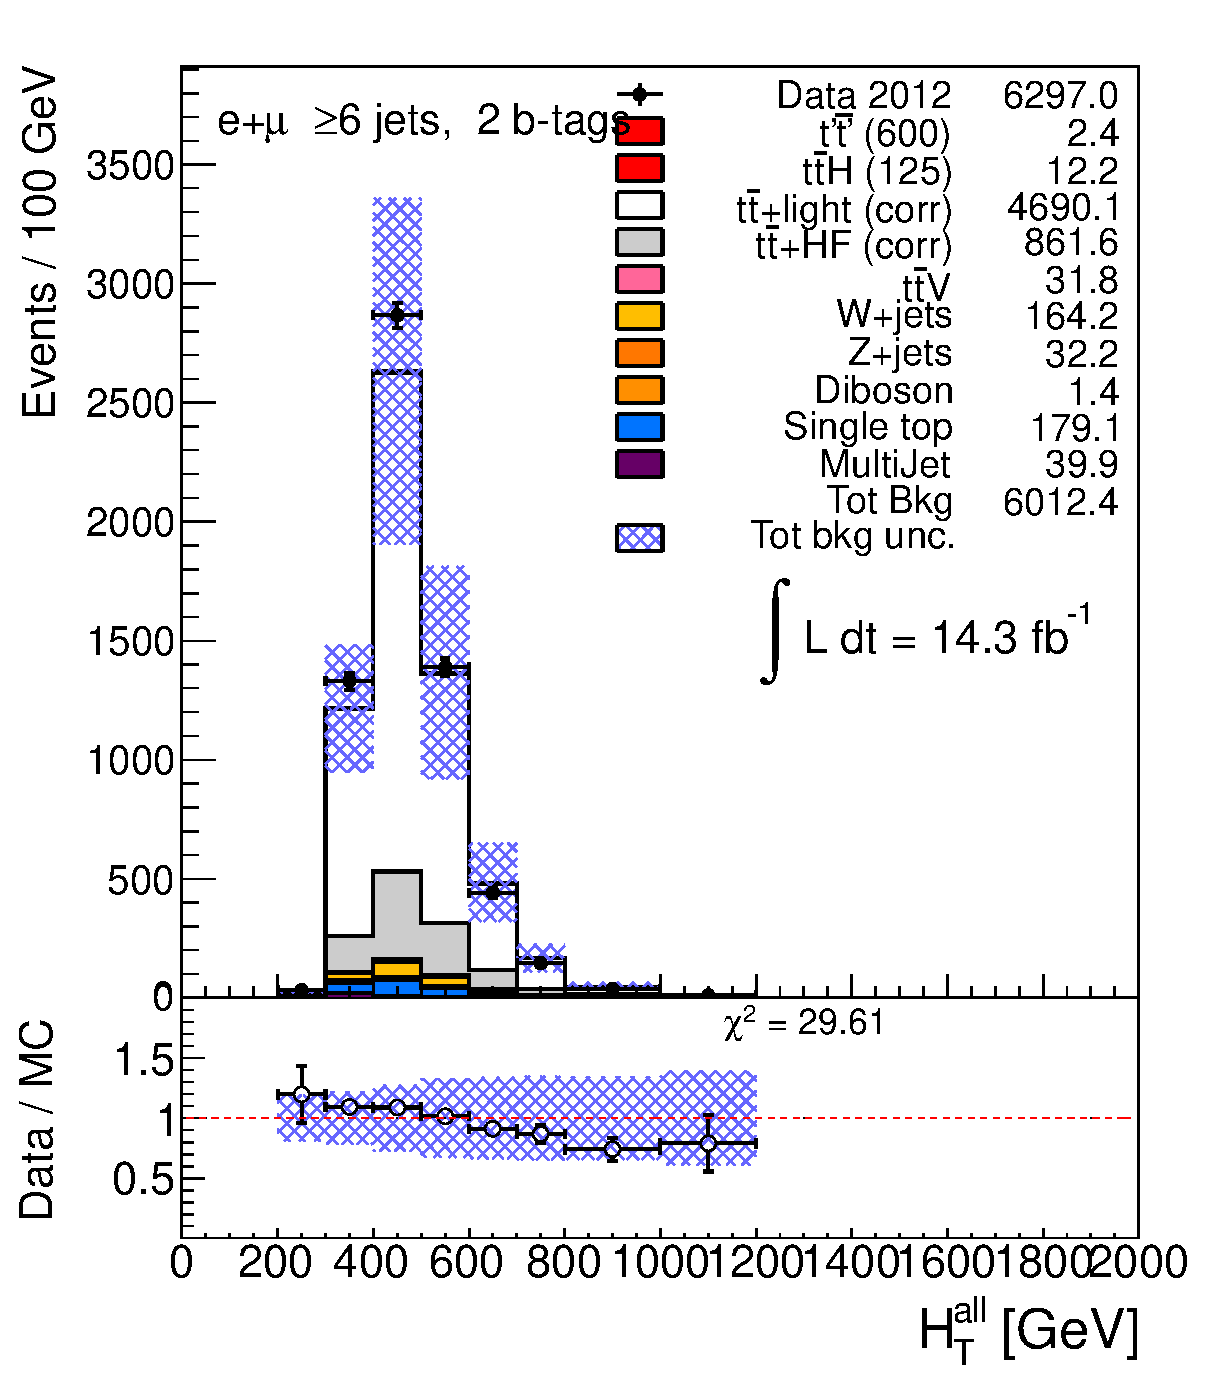
\includegraphics[width=0.30\textwidth]{figures/controlRegionsHTTail/HTAll_ELEMUON_6jetin2btagex_NOMINAL.eps} &
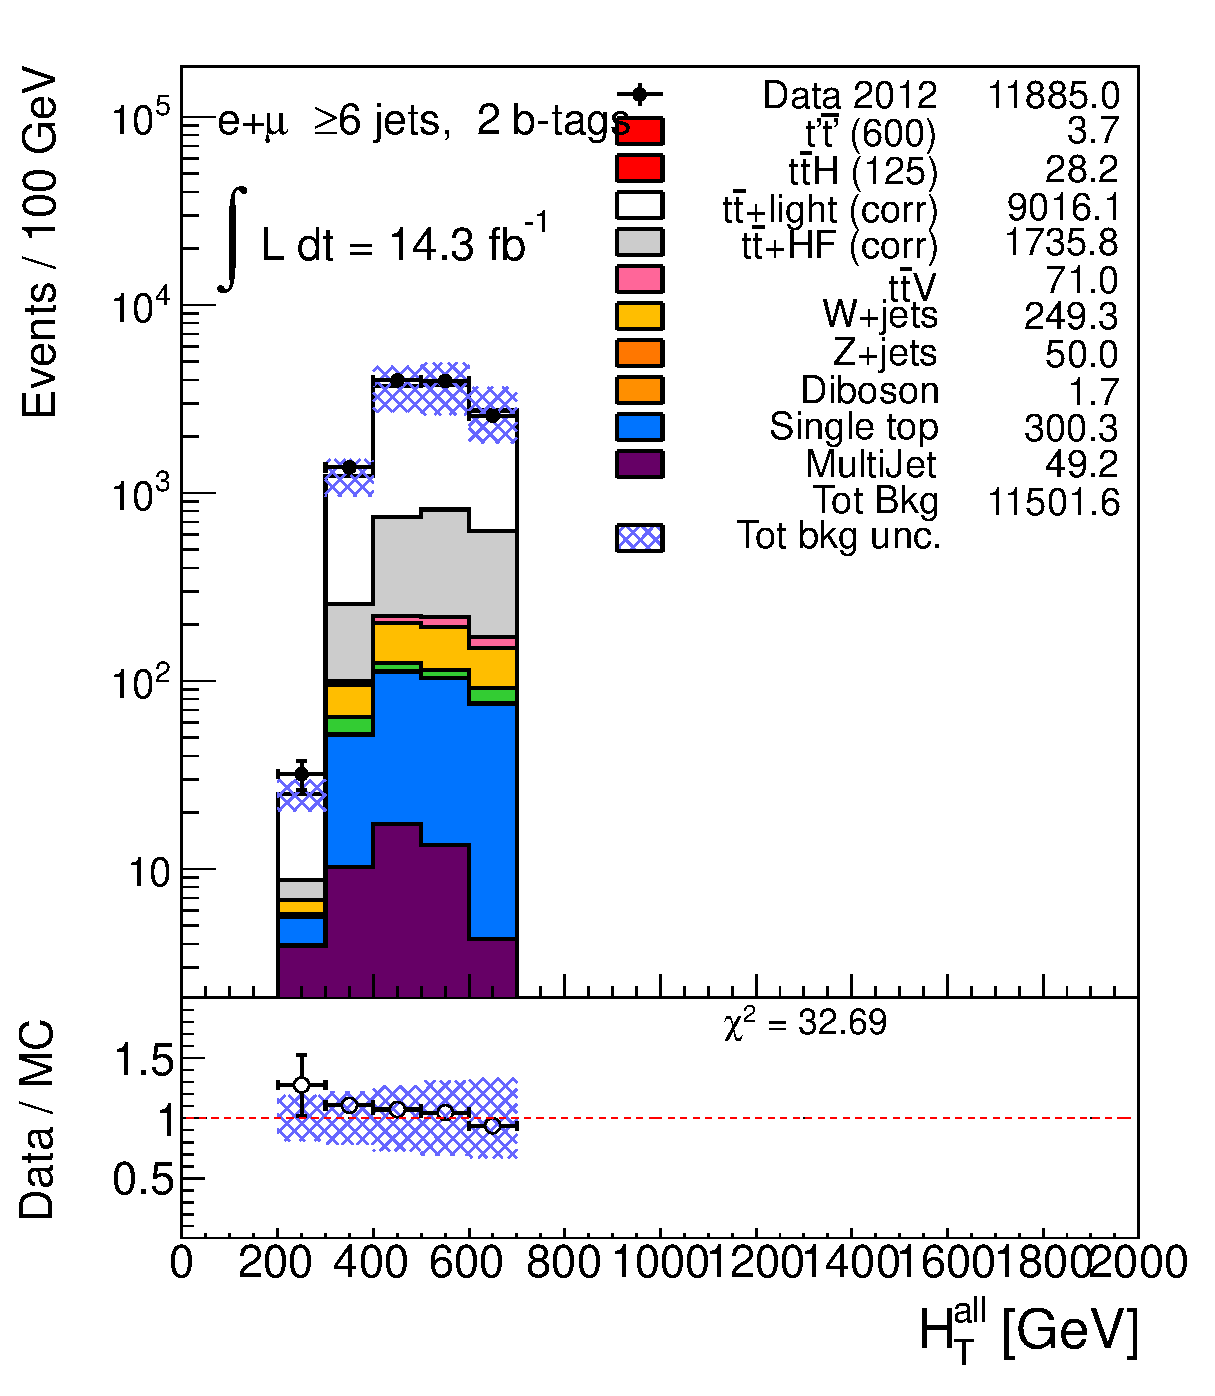
\includegraphics[width=0.30\textwidth]{figures/controlRegionsHTTail/HTAll_ELEMUON_6jetin2btagex_NOMINAL_logscale.eps} \\
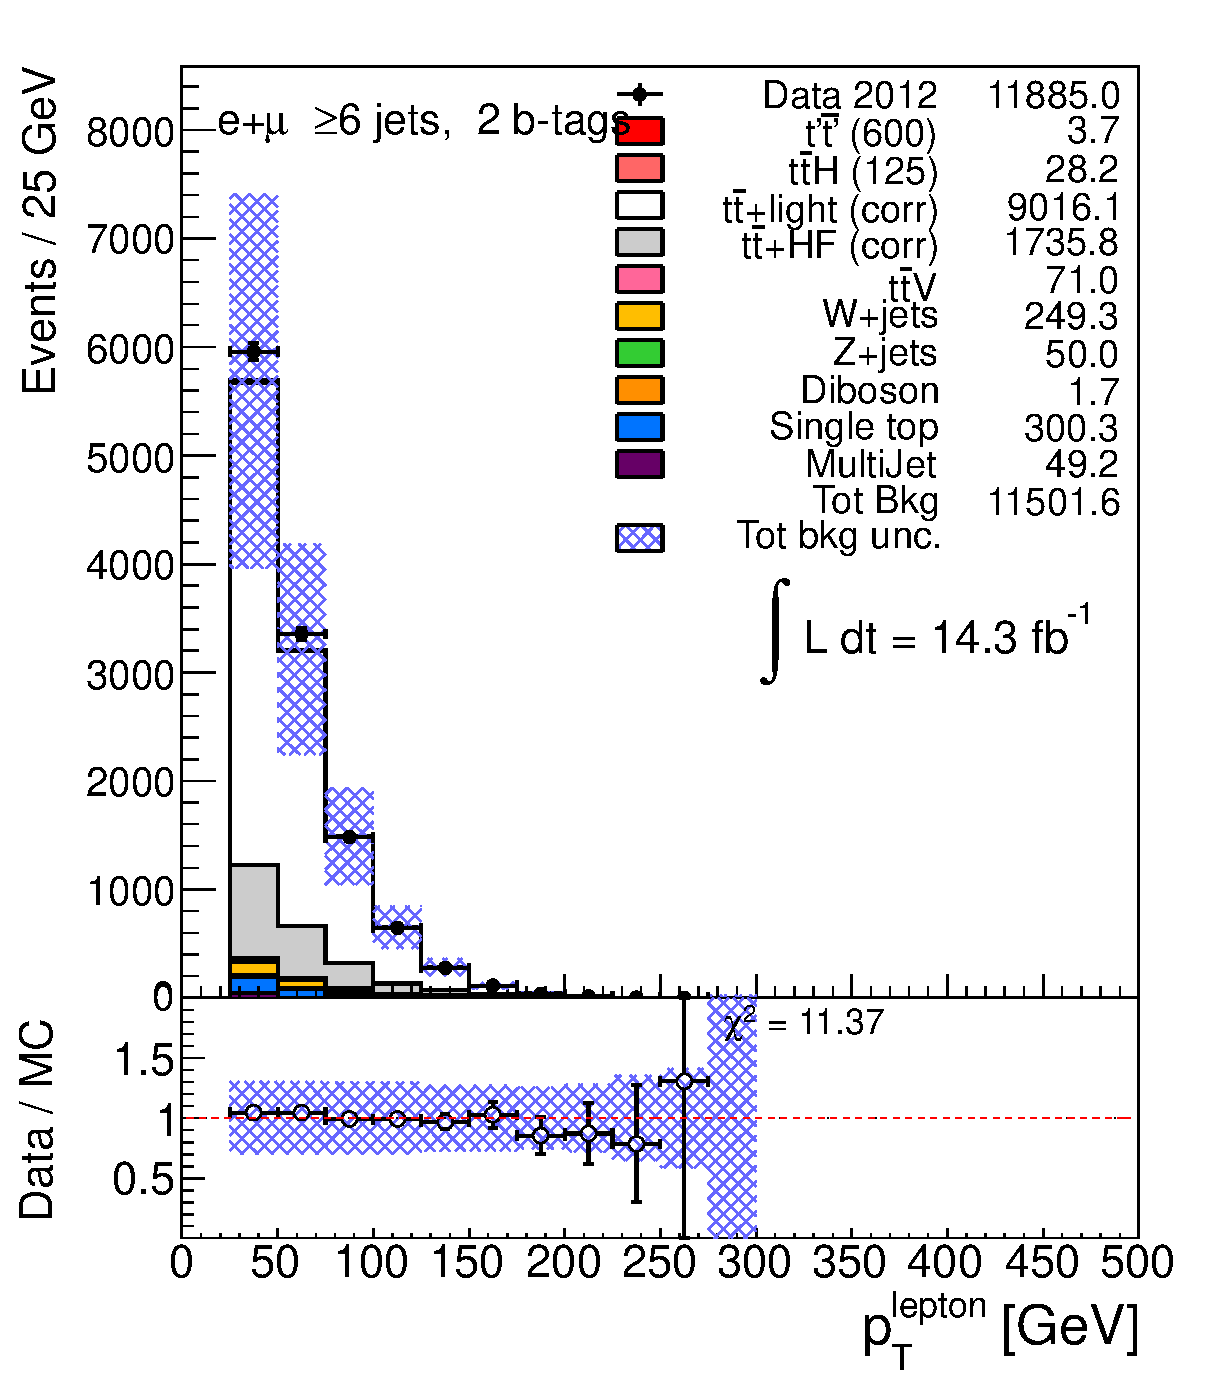
\includegraphics[width=0.30\textwidth]{figures/controlRegionsHTTail/LepPt_ELEMUON_6jetin2btagex_NOMINAL.eps} &
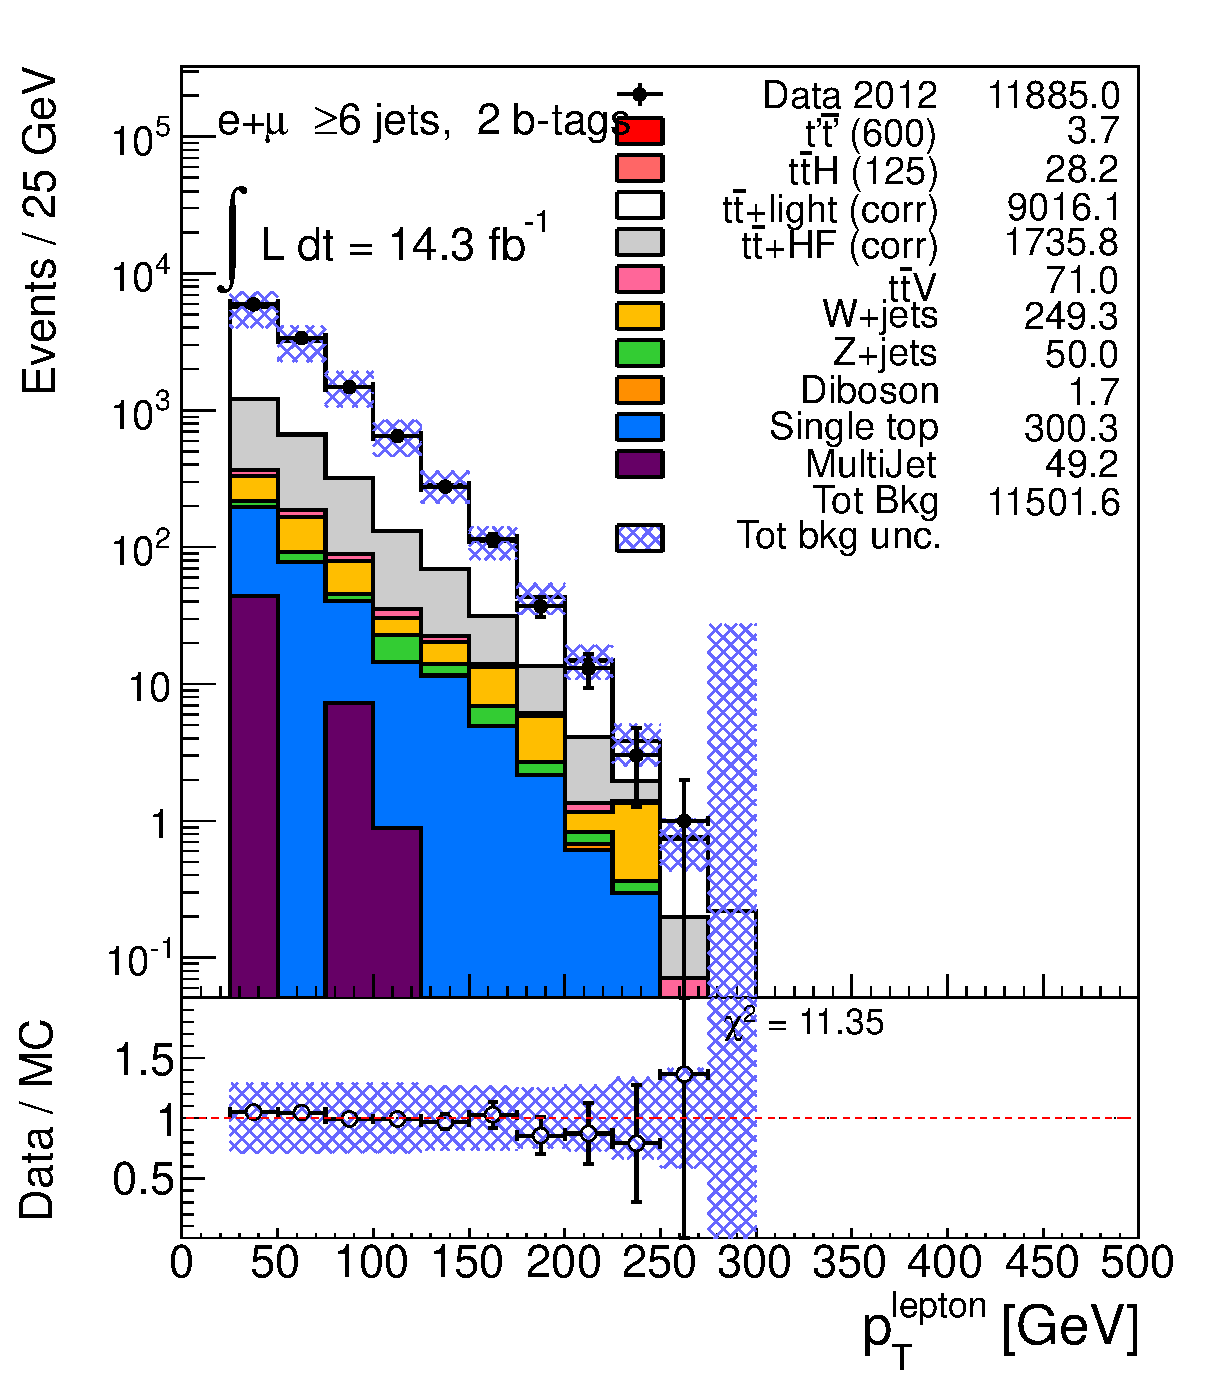
\includegraphics[width=0.30\textwidth]{figures/controlRegionsHTTail/LepPt_ELEMUON_6jetin2btagex_NOMINAL_logscale.eps} \\
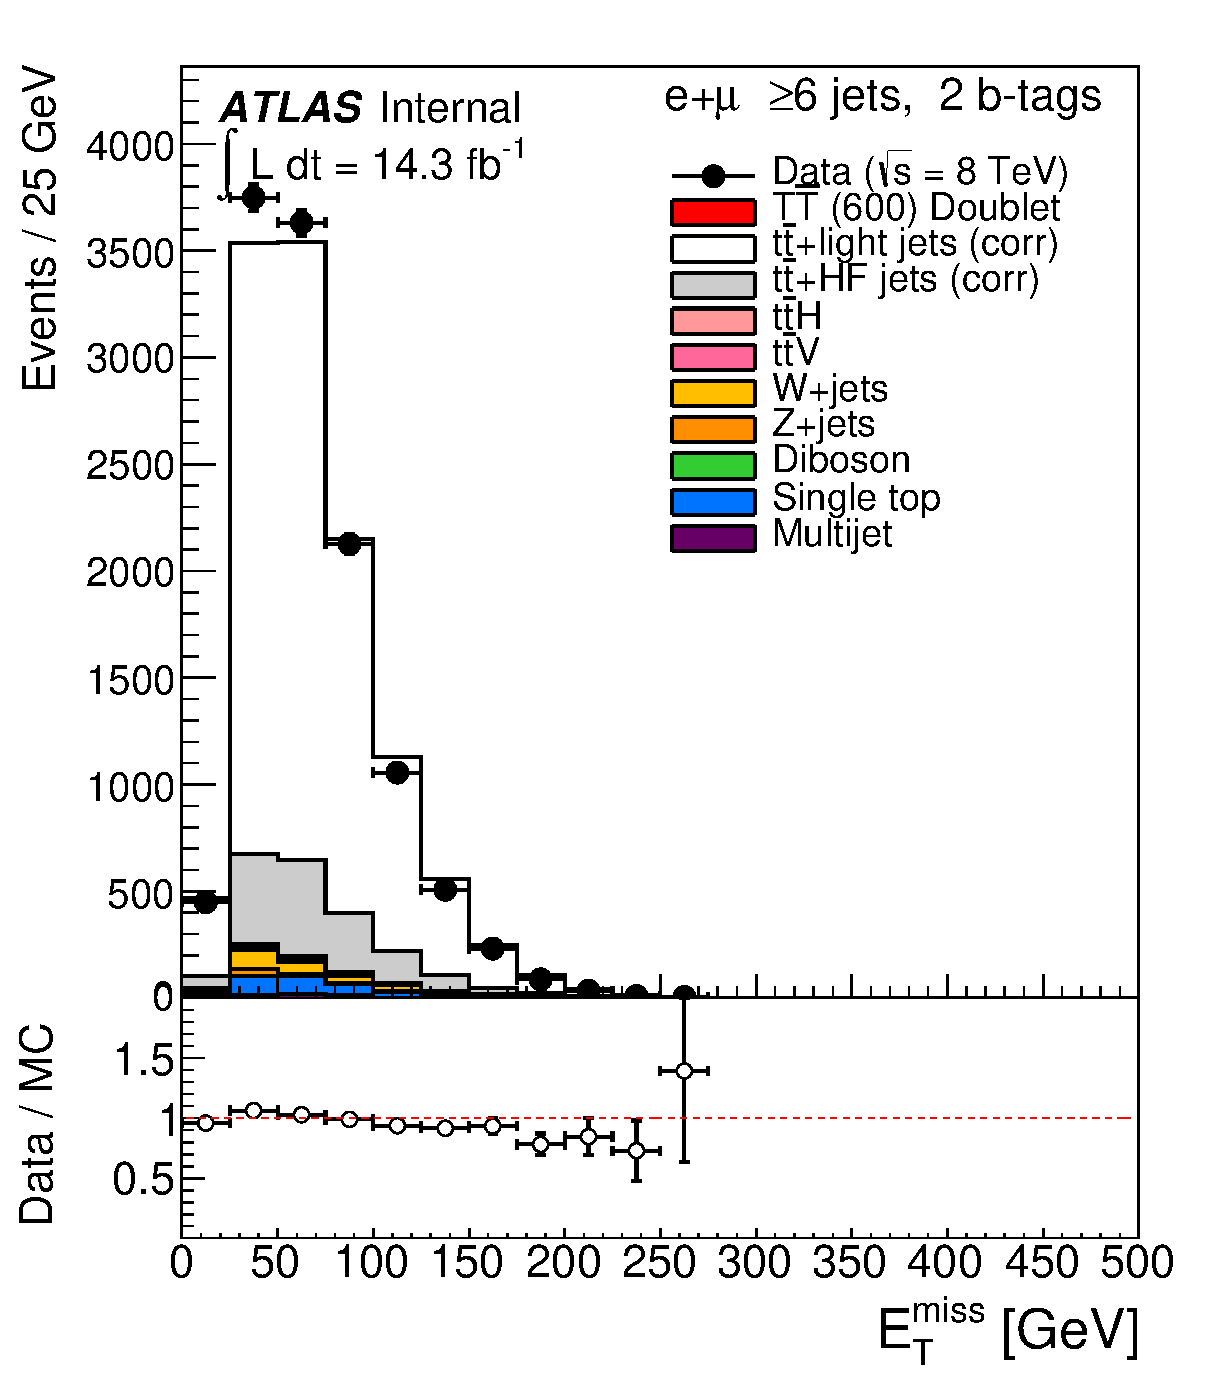
\includegraphics[width=0.30\textwidth]{figures/controlRegionsHTTail/MET_ELEMUON_6jetin2btagex_NOMINAL.eps} &
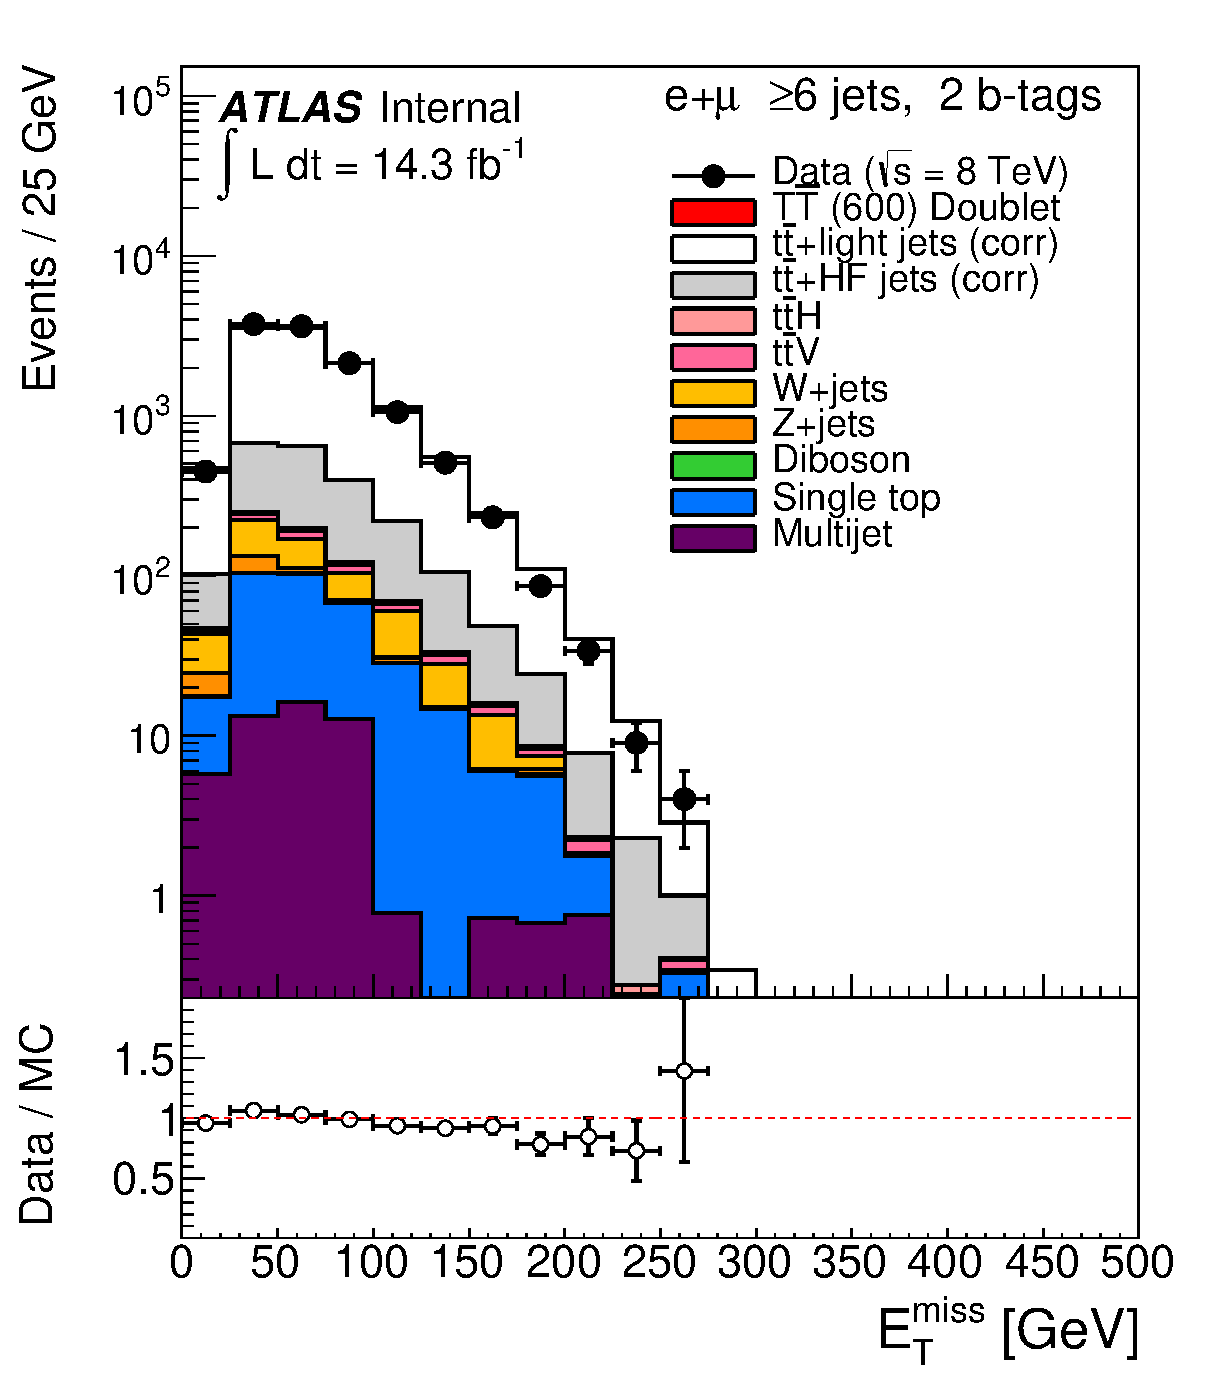
\includegraphics[width=0.30\textwidth]{figures/controlRegionsHTTail/MET_ELEMUON_6jetin2btagex_NOMINAL_logscale.eps} \\
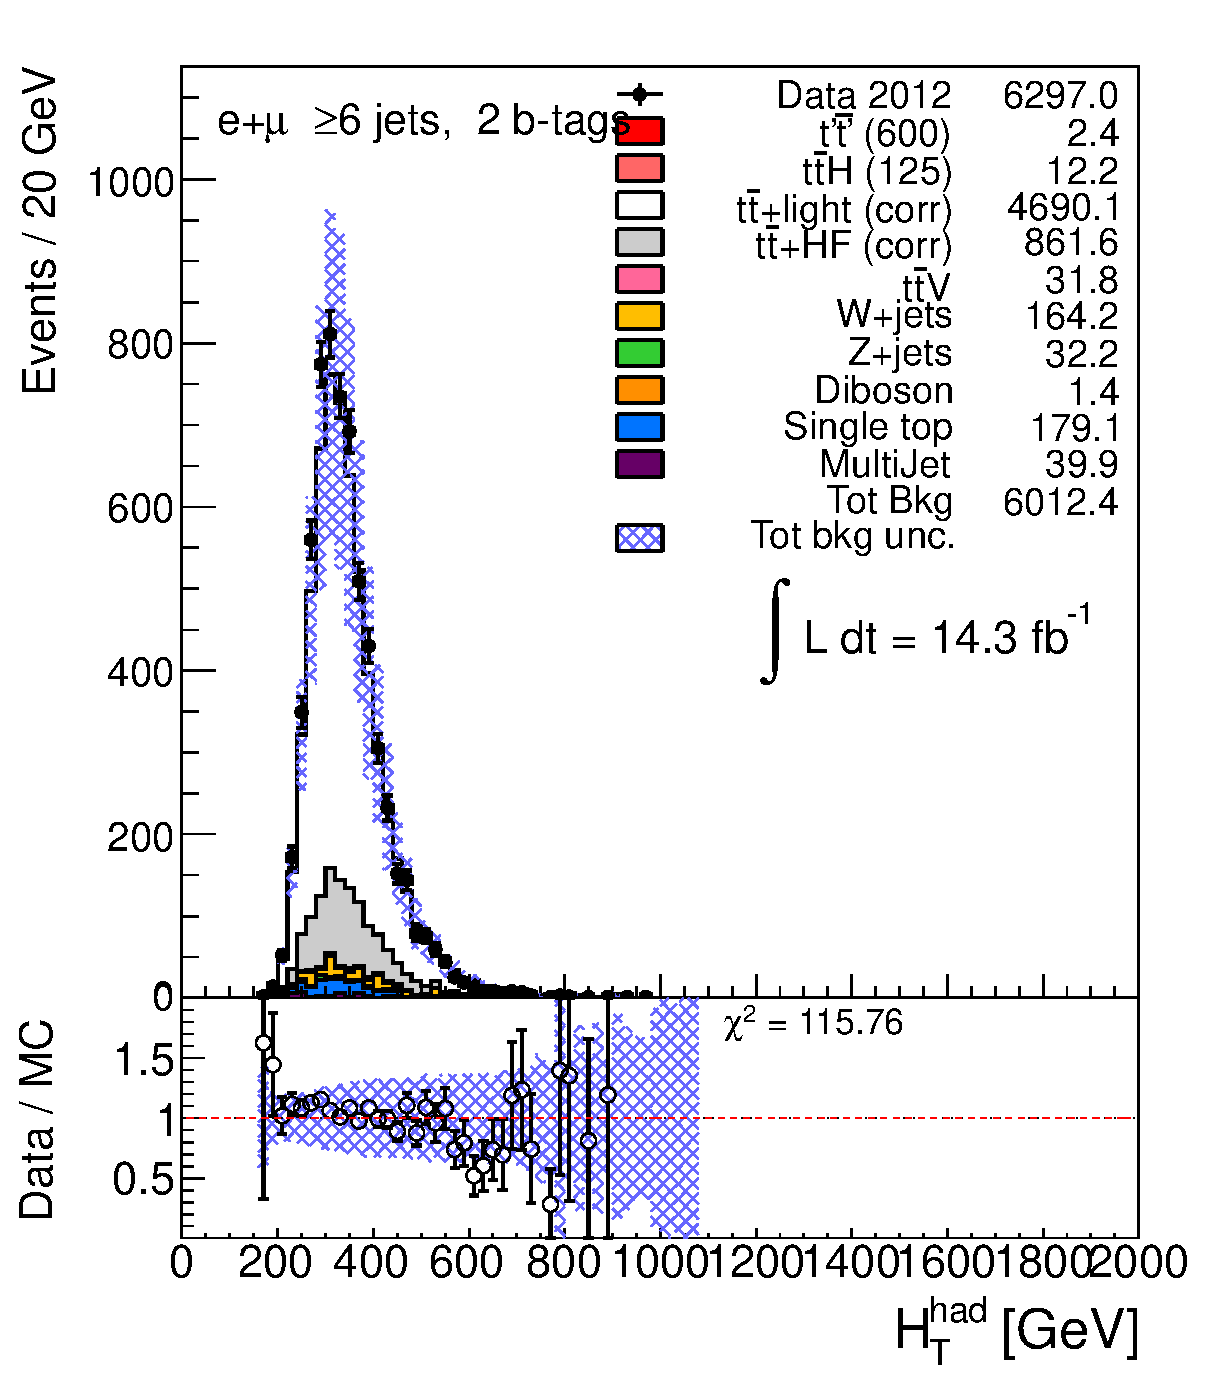
\includegraphics[width=0.30\textwidth]{figures/controlRegionsHTTail/HTHad_ELEMUON_6jetin2btagex_NOMINAL.eps} &
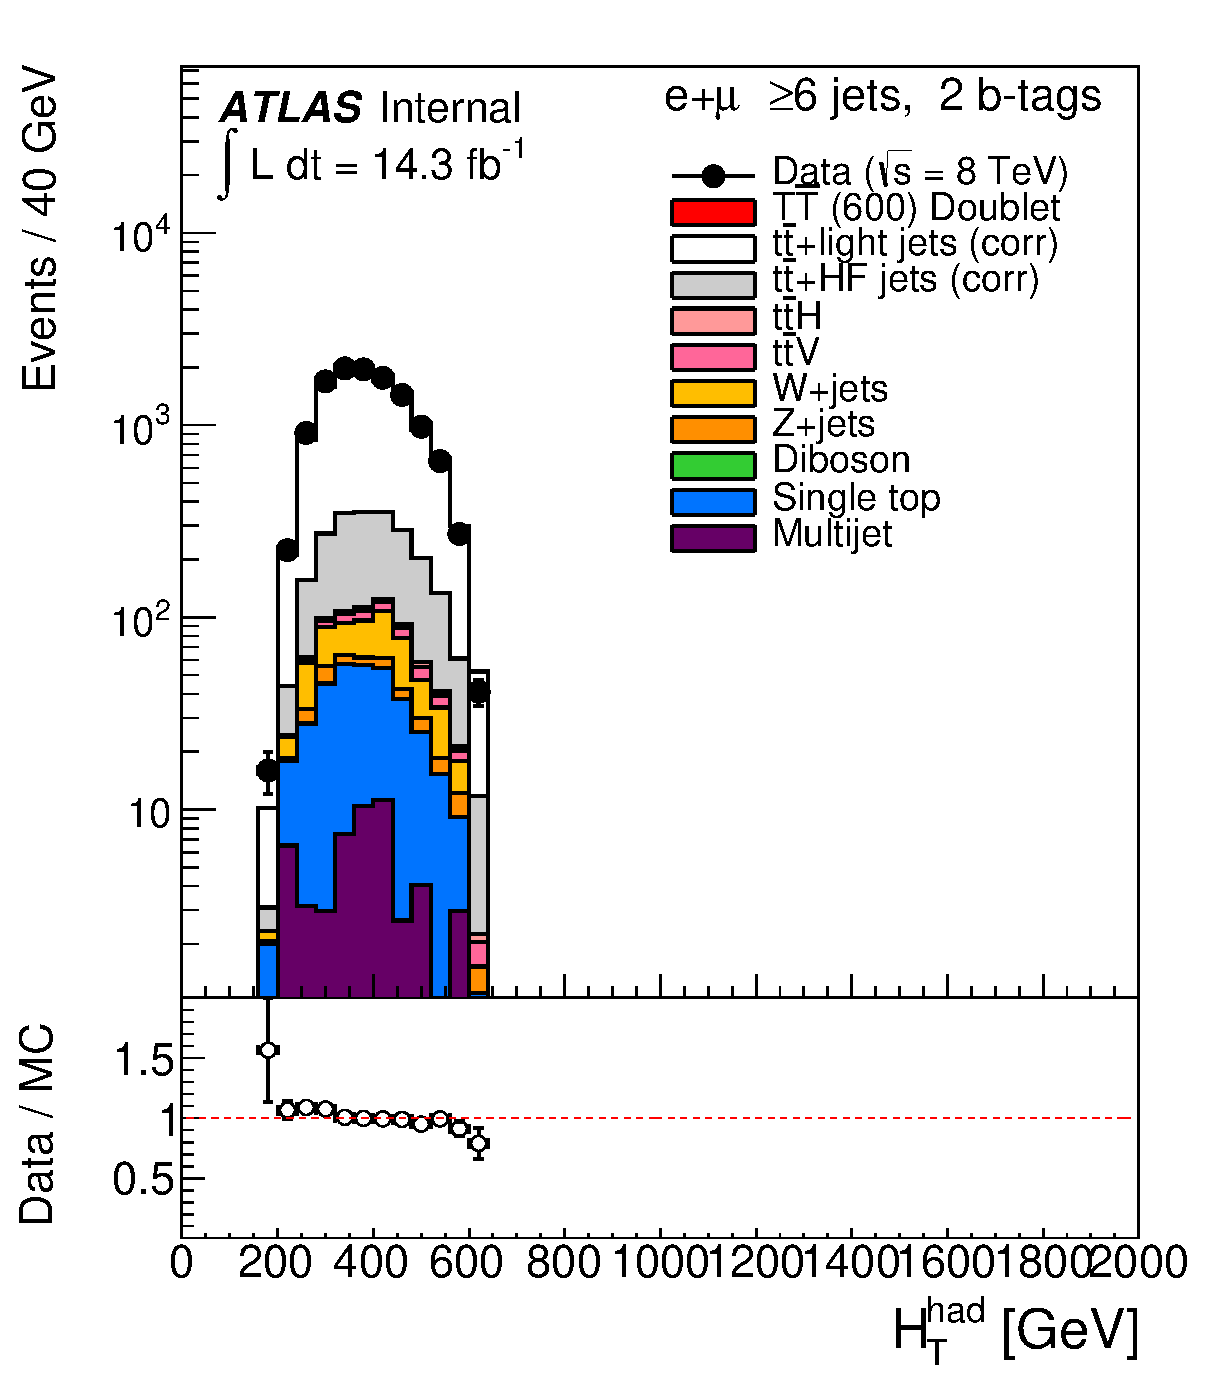
\includegraphics[width=0.30\textwidth]{figures/controlRegionsHTTail/HTHad_ELEMUON_6jetin2btagex_NOMINAL_logscale.eps} \\

\end{tabular}\caption{\small {Comparison between data and prediction in the combined $e$+jets and $\mu$+jets channels with 2 $b$-tagged jets in the control sample
defined to study the high $\HT$ tail (see text for details)  for a number of kinematic
variables. From top to bottom, the variables displayed are: $\HT$, and its basic ingredients, lepton $\pt$, $\met$ and $\hthad$,
in (left) linear scale and (right) logarithmic scale.
The shaded area represents the pre-fit total background uncertainty.}}
\label{fig:ELEMUON_controlHTTail_2btagex_1}
\end{center}
\end{figure}
%%%%%%%%%%%%%%
%%%%%%%%%%%%%%
\begin{figure}[htbp]
\begin{center}
\begin{tabular}{cc}
%
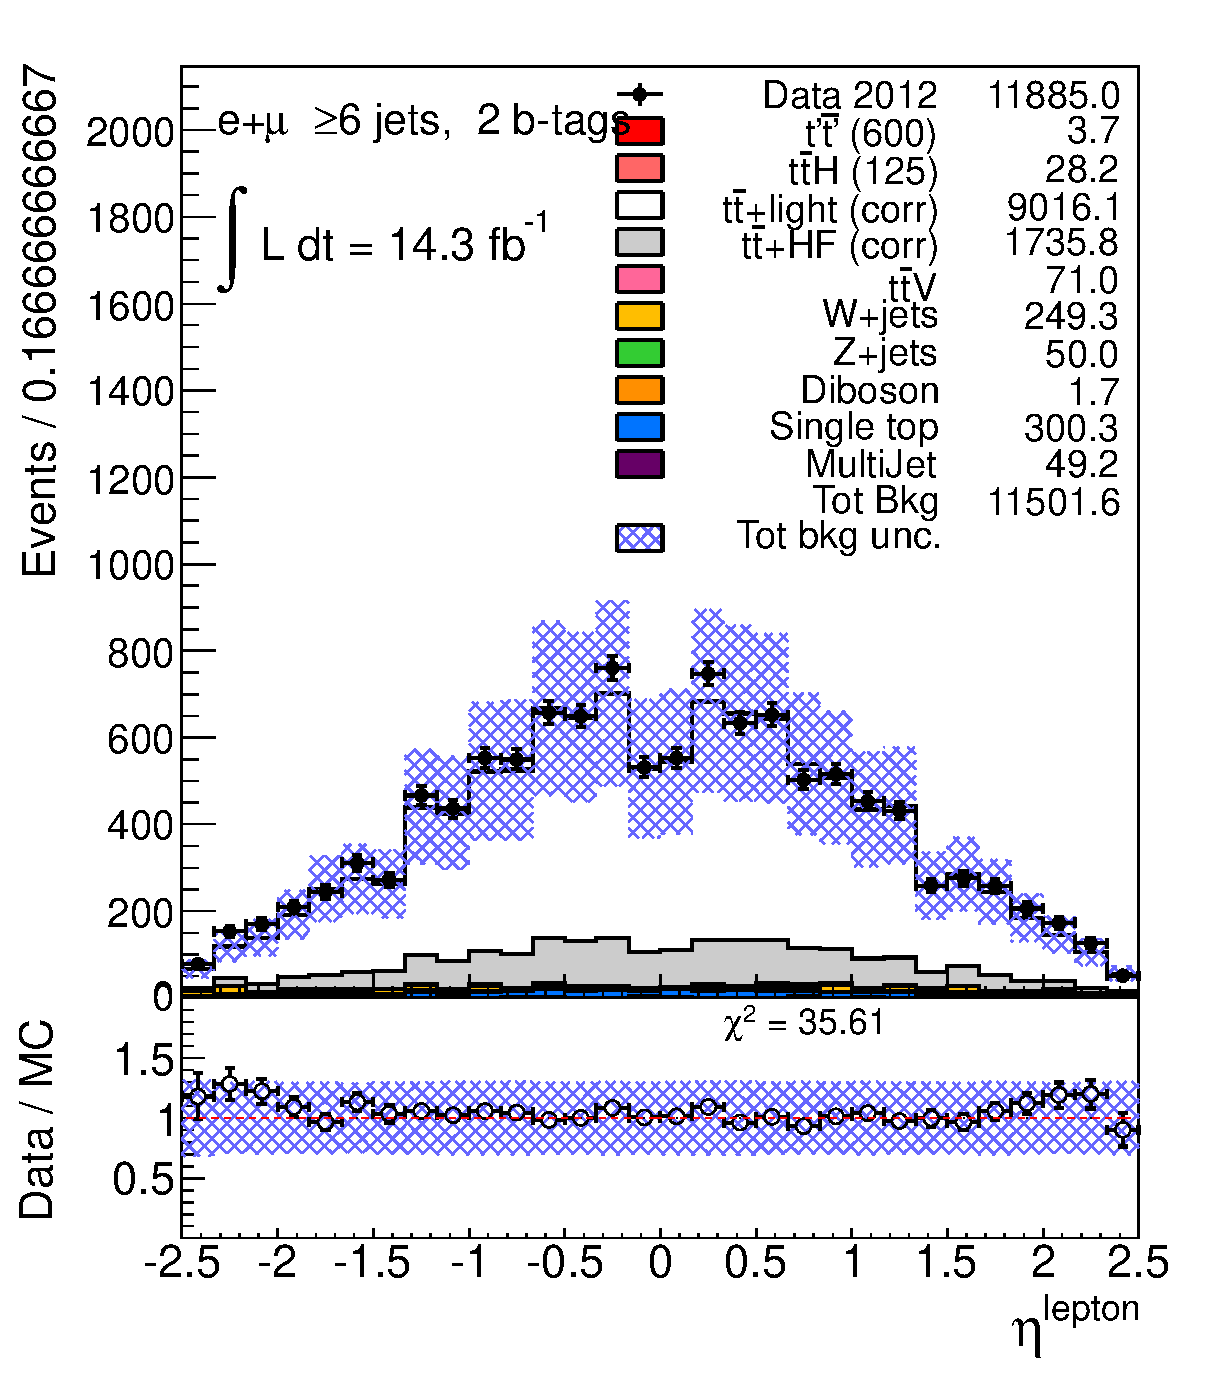
\includegraphics[width=0.30\textwidth]{figures/controlRegionsHTTail/LepEta_ELEMUON_6jetin2btagex_NOMINAL.eps} &
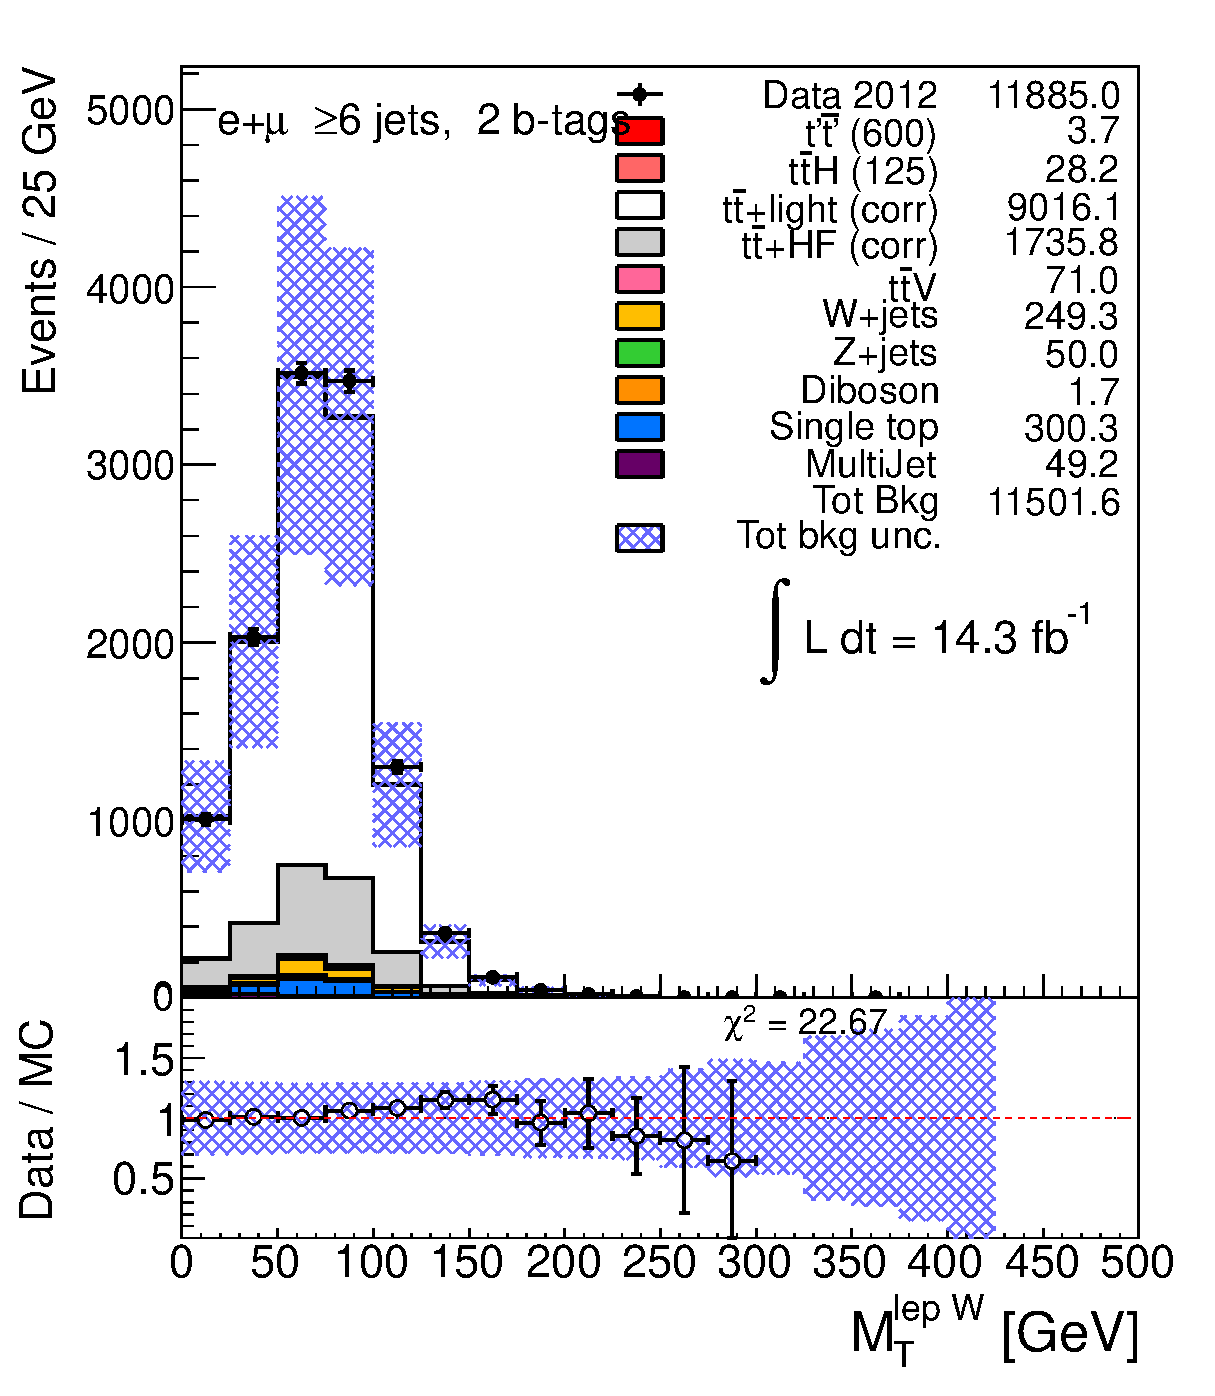
\includegraphics[width=0.30\textwidth]{figures/controlRegionsHTTail/Wlep_MassT_ELEMUON_6jetin2btagex_NOMINAL.eps} \\
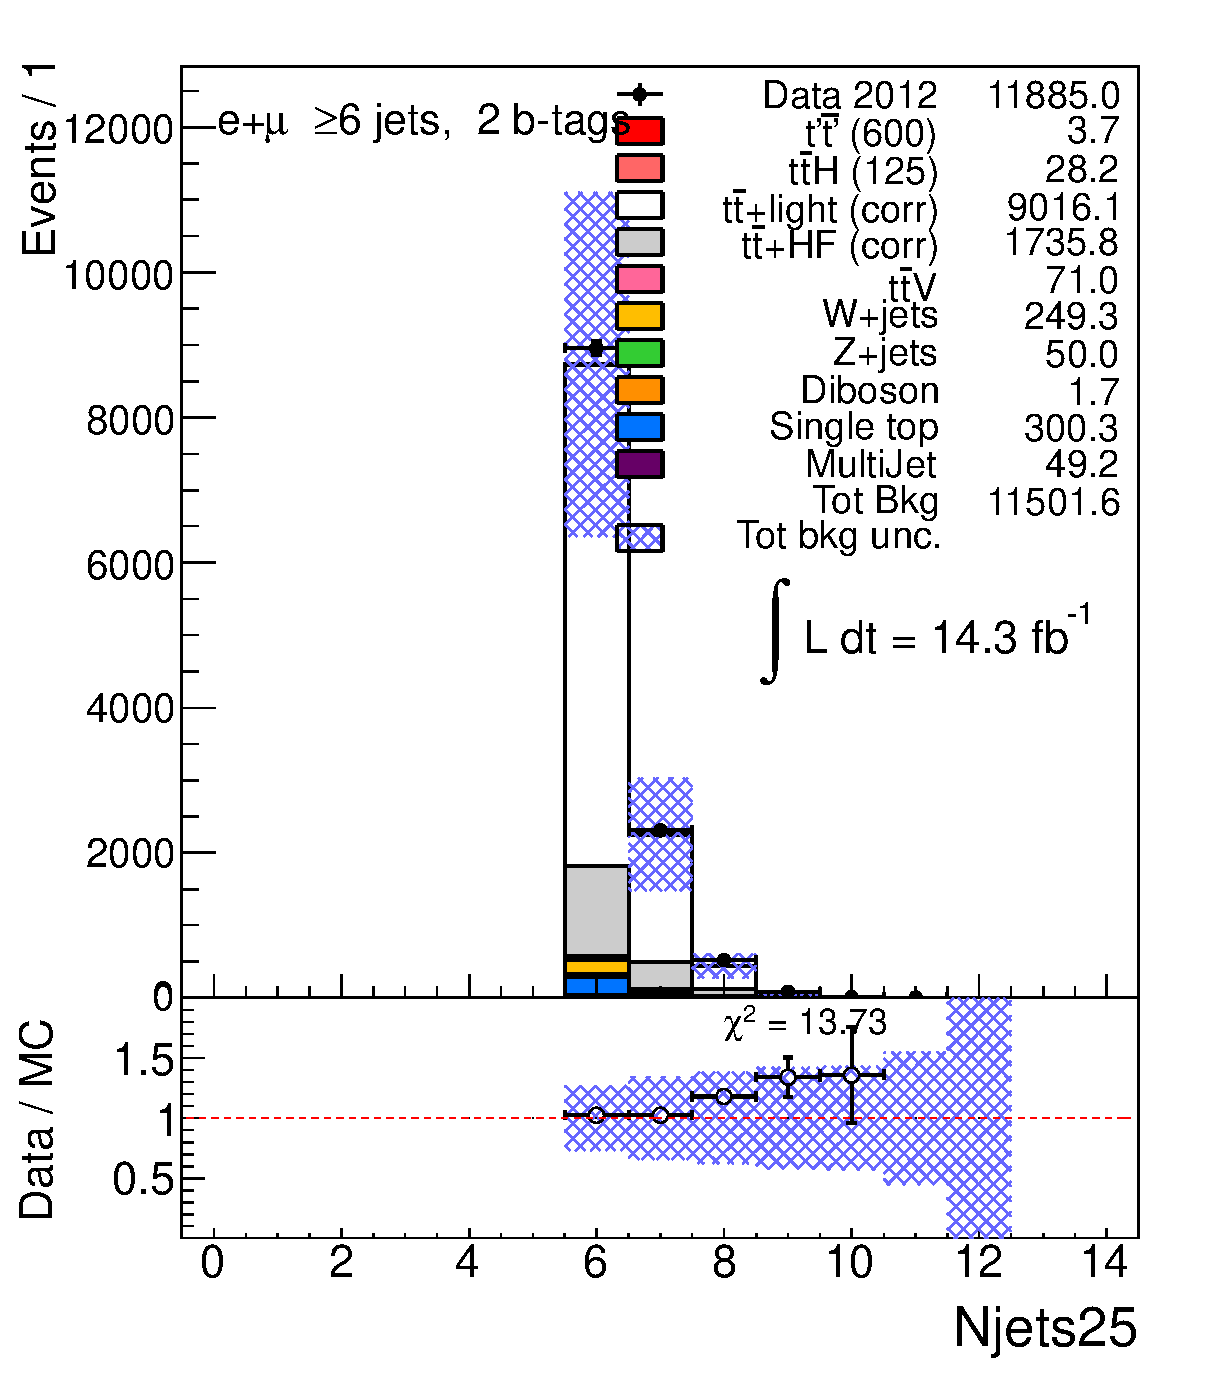
\includegraphics[width=0.30\textwidth]{figures/controlRegionsHTTail/Njets25_ELEMUON_6jetin2btagex_NOMINAL.eps} &
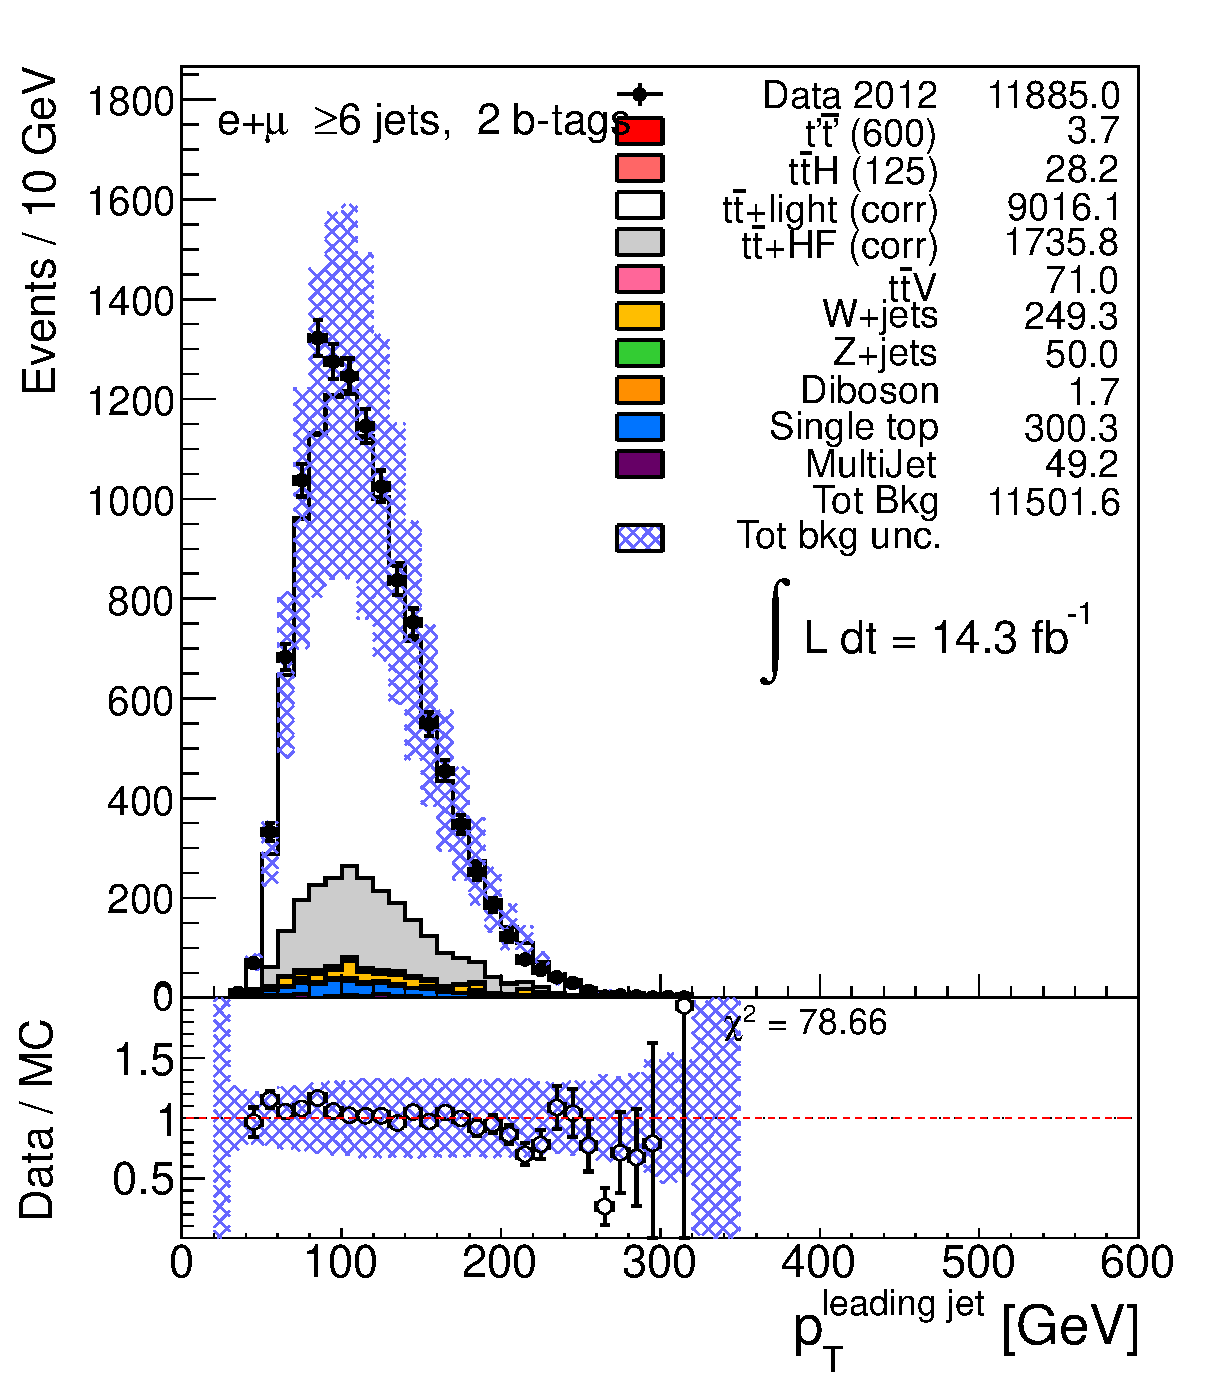
\includegraphics[width=0.30\textwidth]{figures/controlRegionsHTTail/JetPt1_ELEMUON_6jetin2btagex_NOMINAL.eps} \\
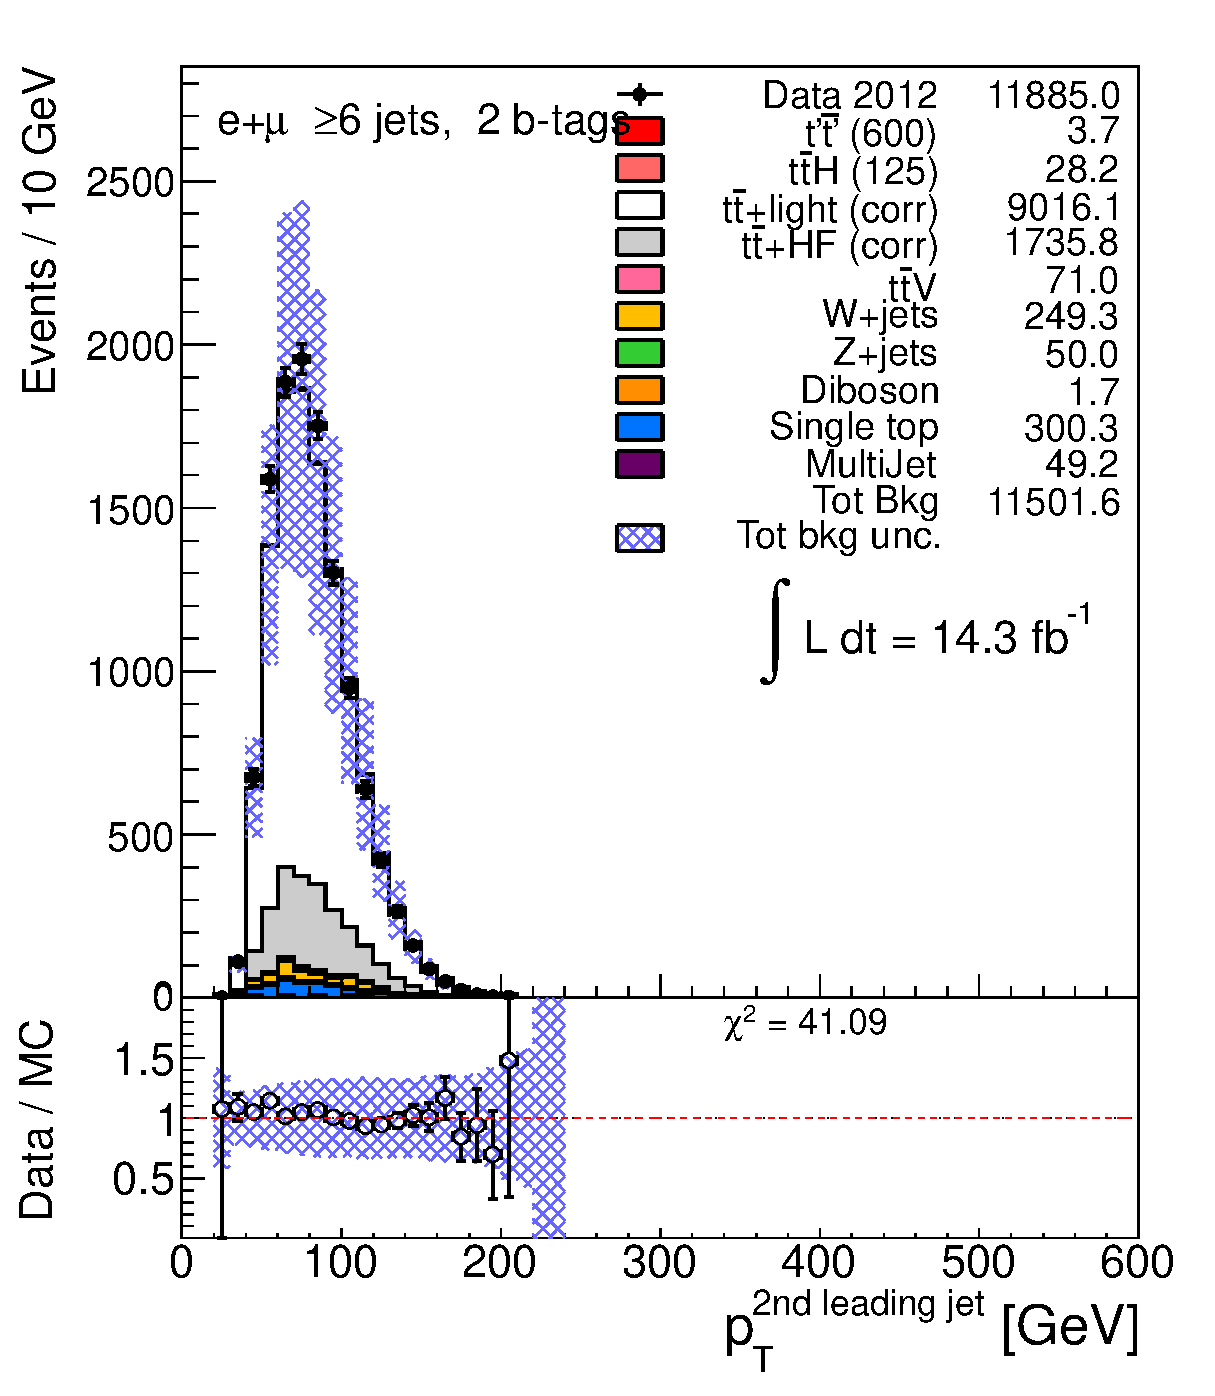
\includegraphics[width=0.30\textwidth]{figures/controlRegionsHTTail/JetPt2_ELEMUON_6jetin2btagex_NOMINAL.eps} &
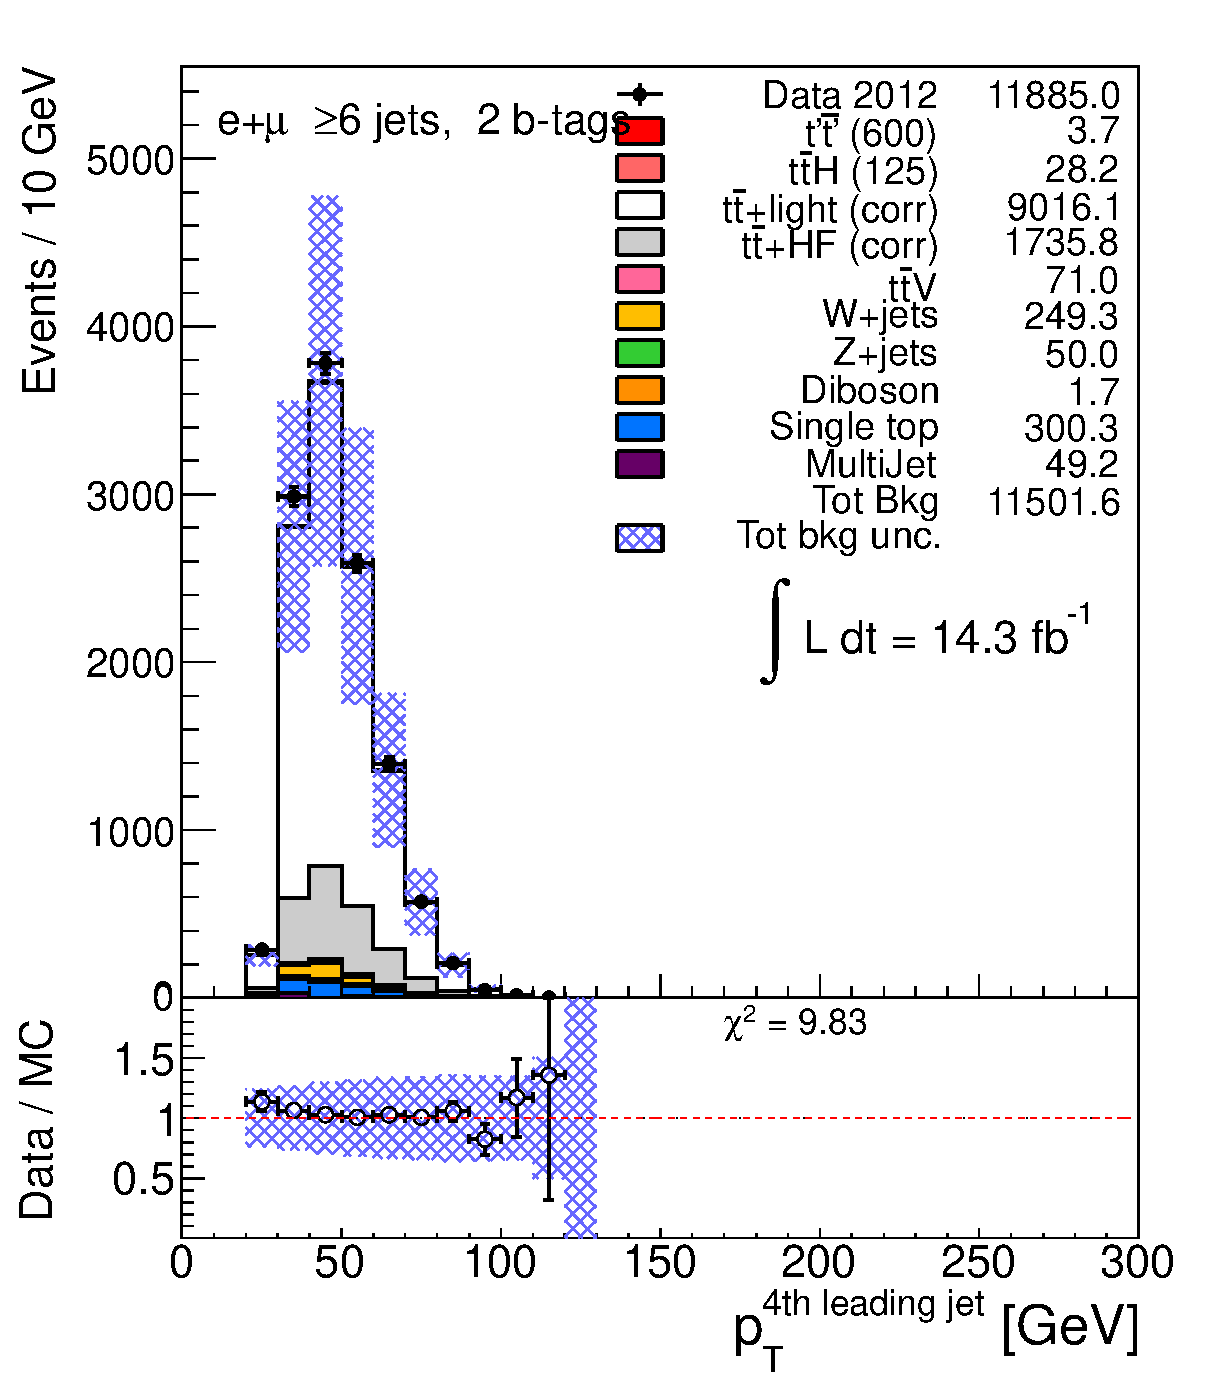
\includegraphics[width=0.30\textwidth]{figures/controlRegionsHTTail/JetPt4_ELEMUON_6jetin2btagex_NOMINAL.eps} \\
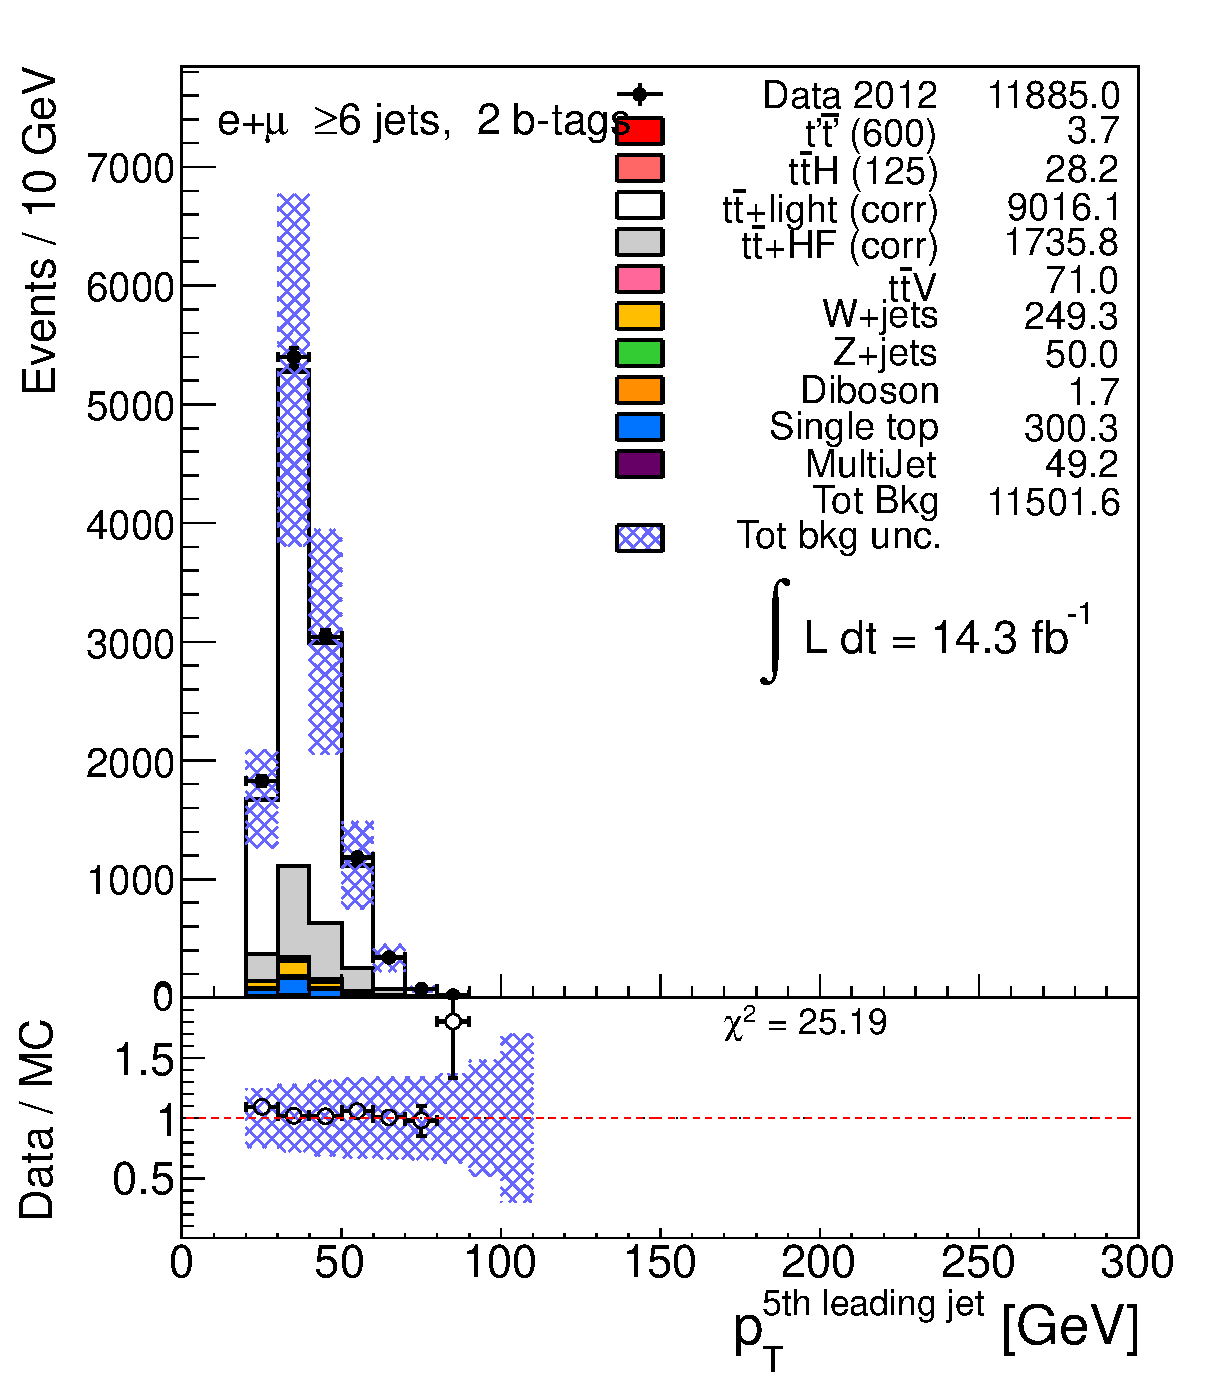
\includegraphics[width=0.30\textwidth]{figures/controlRegionsHTTail/JetPt5_ELEMUON_6jetin2btagex_NOMINAL.eps} &
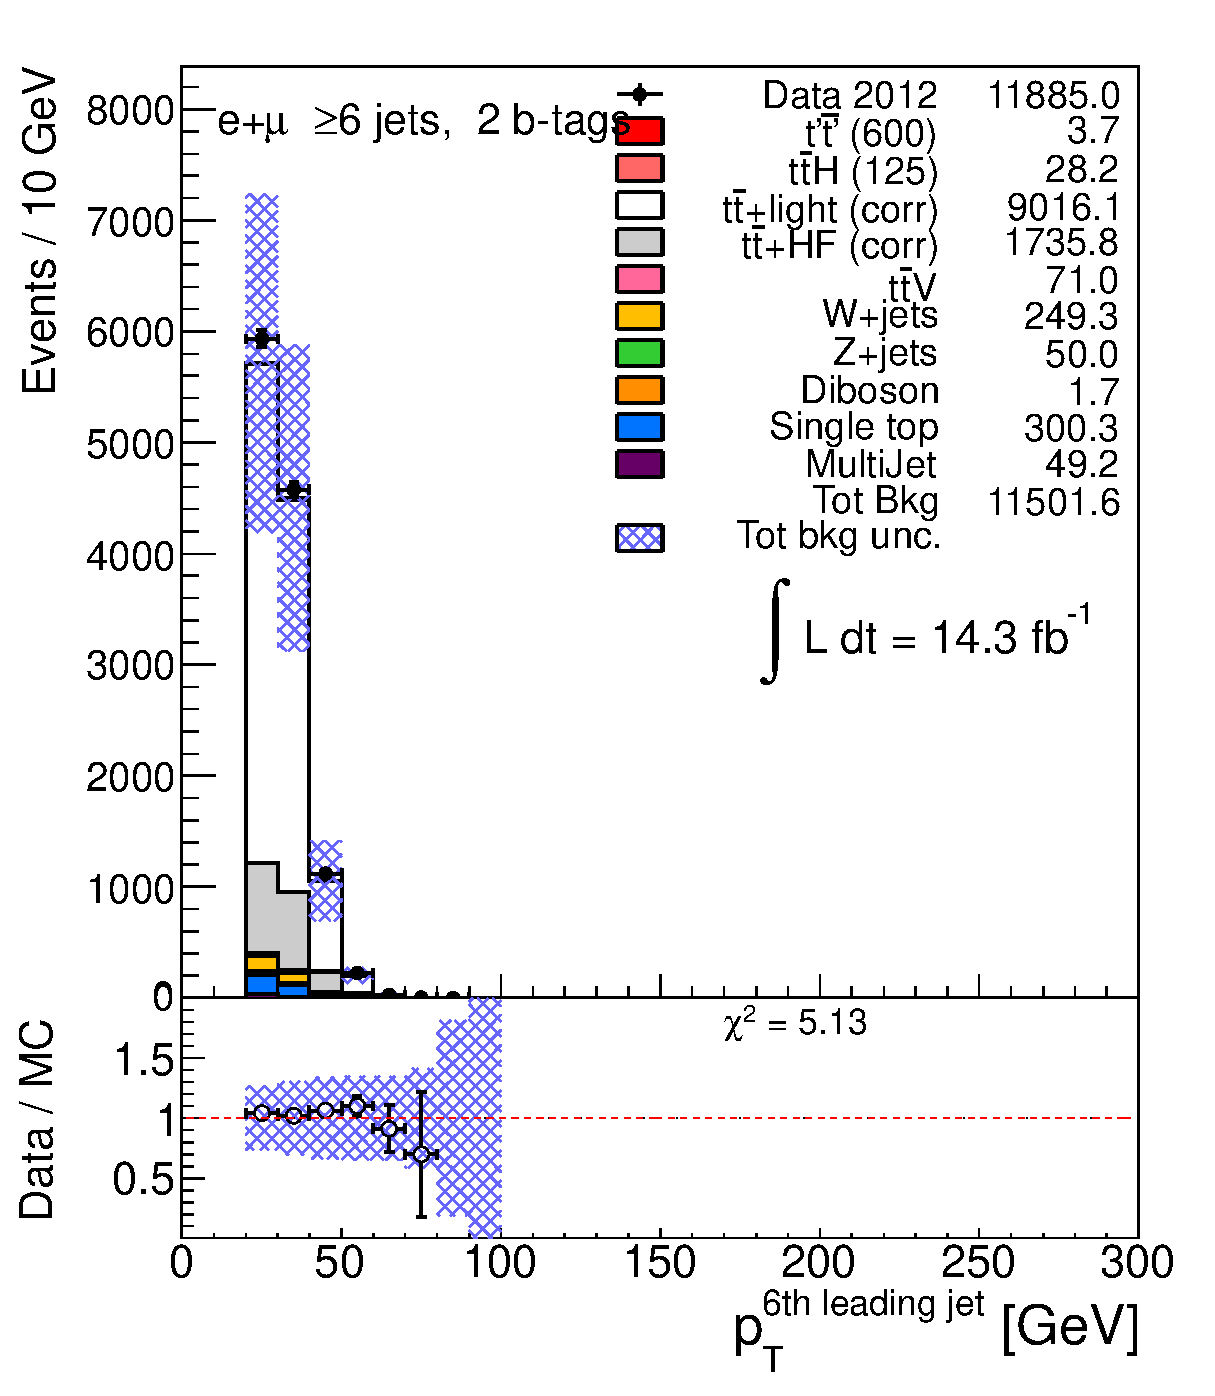
\includegraphics[width=0.30\textwidth]{figures/controlRegionsHTTail/JetPt6_ELEMUON_6jetin2btagex_NOMINAL.eps} \\
\end{tabular}\caption{\small {Comparison between data and prediction in the combined $e$+jets and $\mu$+jets channels with 2 $b$-tagged jets in the control sample
defined to study the high $\HT$ tail (see text for details)  for a number of kinematic
variables. From top to bottom, and left to right, the variables displayed are: lepton $\eta$, $W$ transverse mass, jet multiplicity with $\pt>25\gev$, 
and jet $\pt$ up to the 6th leading jet.
The shaded area represents the pre-fit total background uncertainty.}}
\label{fig:ELEMUON_controlHTTail_2btagex_2}
\end{center}
\end{figure}
%%%%%%%%%%%%%%

\clearpage
\subsection{Combined $e$+jets and $\mu$+jets, 3 $b$-tags}
\label{sec:ELEMUON_controlHTTail_3tagex}

%%%%%%%%%%%%%%
\begin{figure}[htbp]
\begin{center}
\begin{tabular}{cc}
%
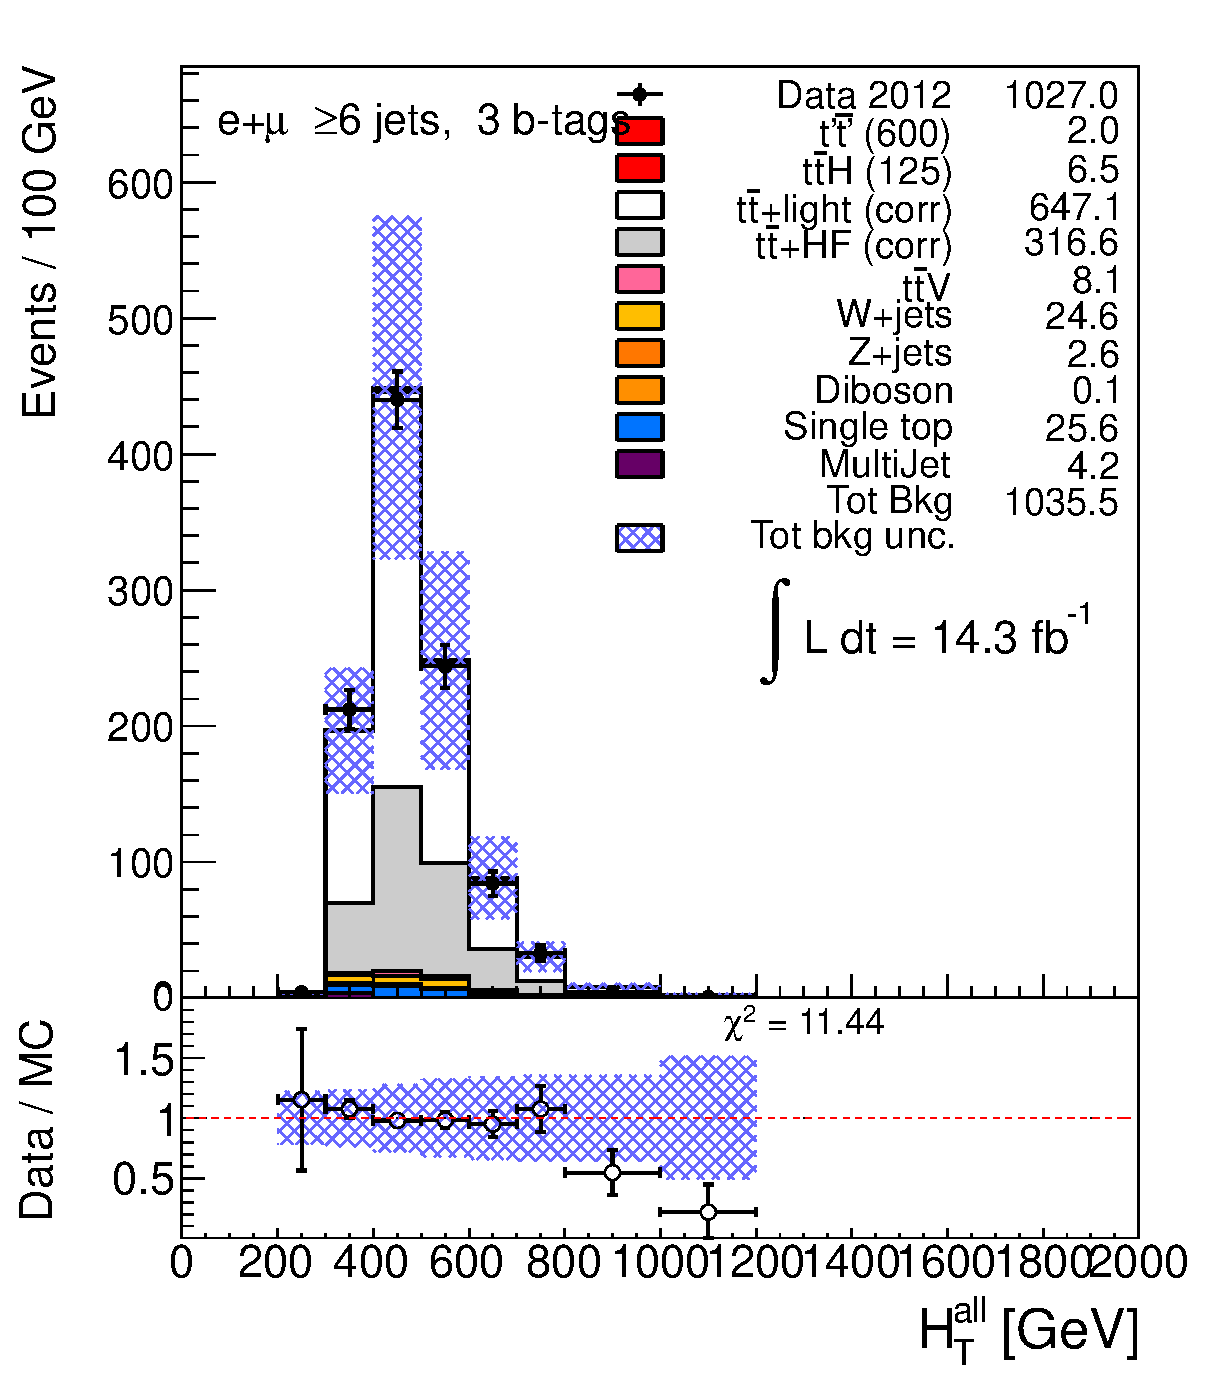
\includegraphics[width=0.30\textwidth]{figures/controlRegionsHTTail/HTAll_ELEMUON_6jetin3btagex_NOMINAL.eps} &
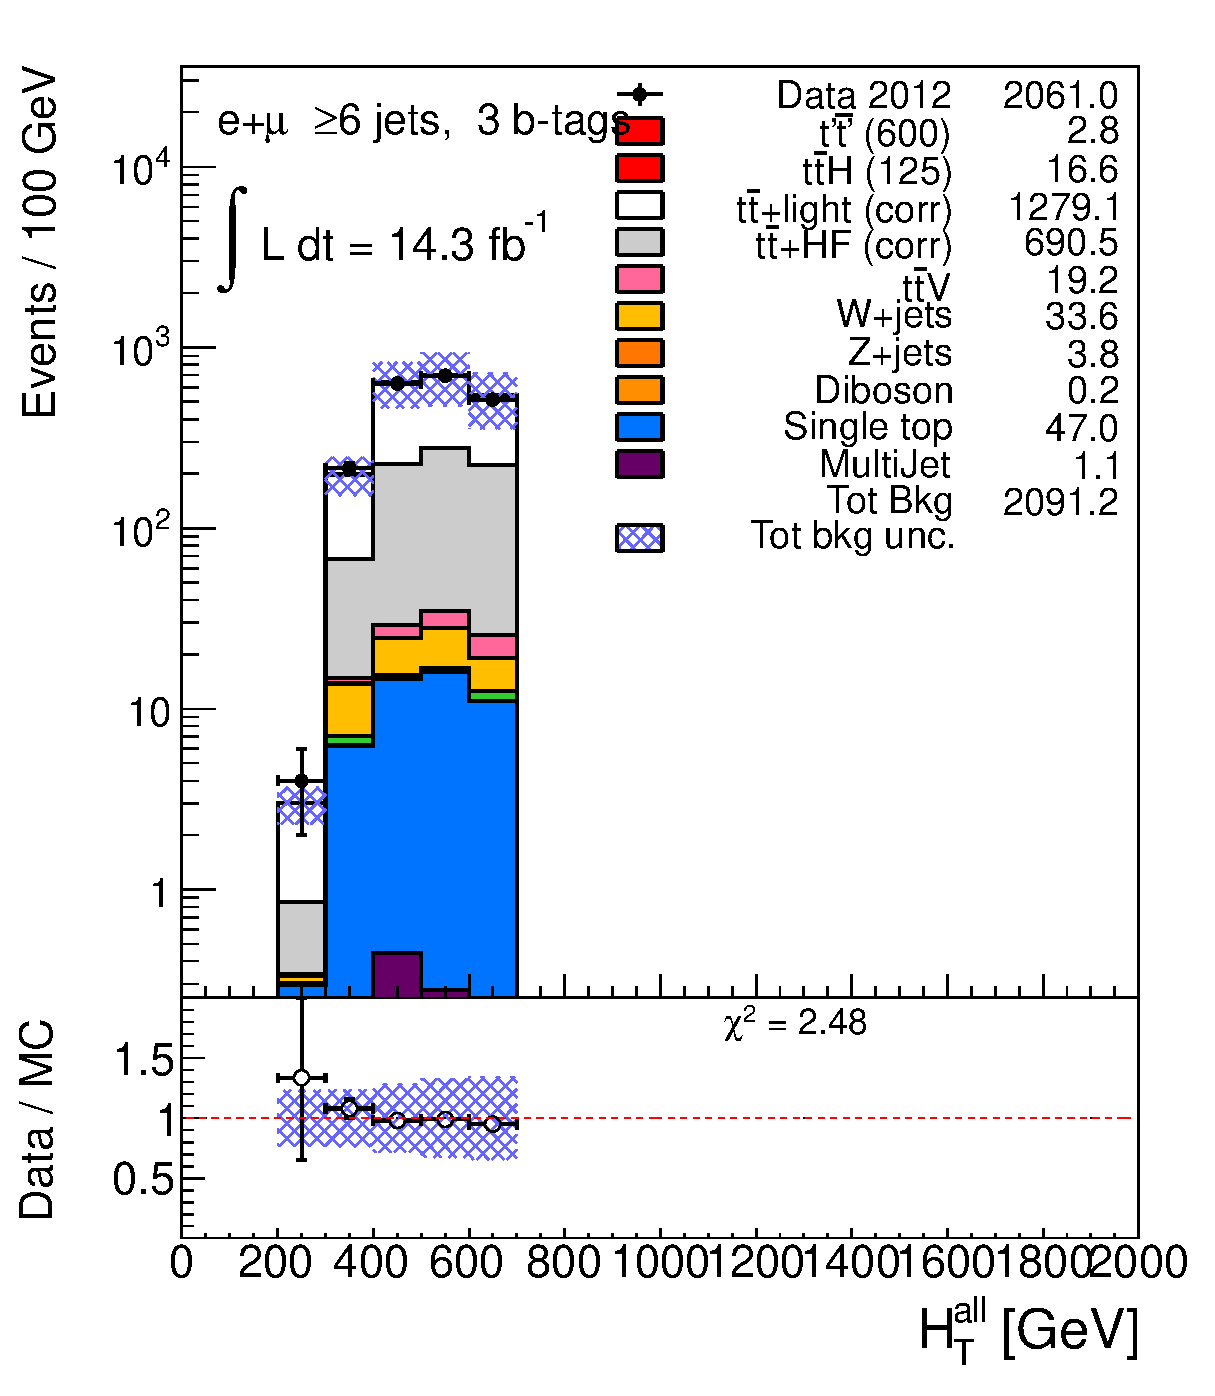
\includegraphics[width=0.30\textwidth]{figures/controlRegionsHTTail/HTAll_ELEMUON_6jetin3btagex_NOMINAL_logscale.eps} \\
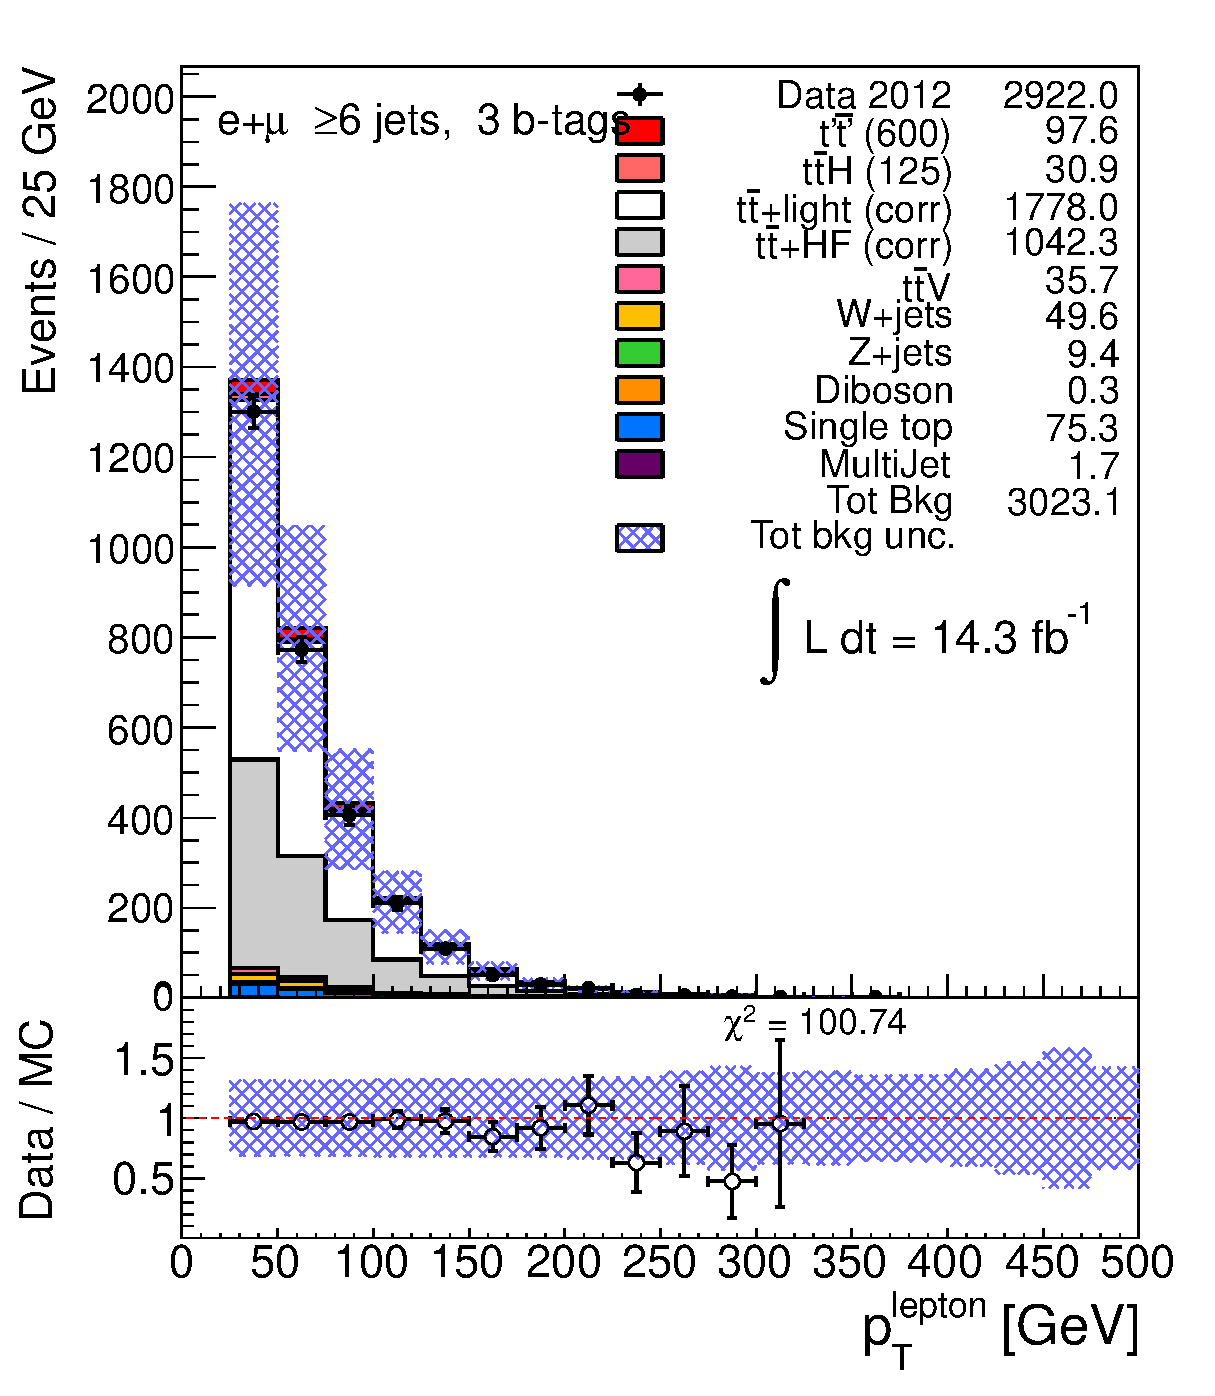
\includegraphics[width=0.30\textwidth]{figures/controlRegionsHTTail/LepPt_ELEMUON_6jetin3btagex_NOMINAL.eps} &
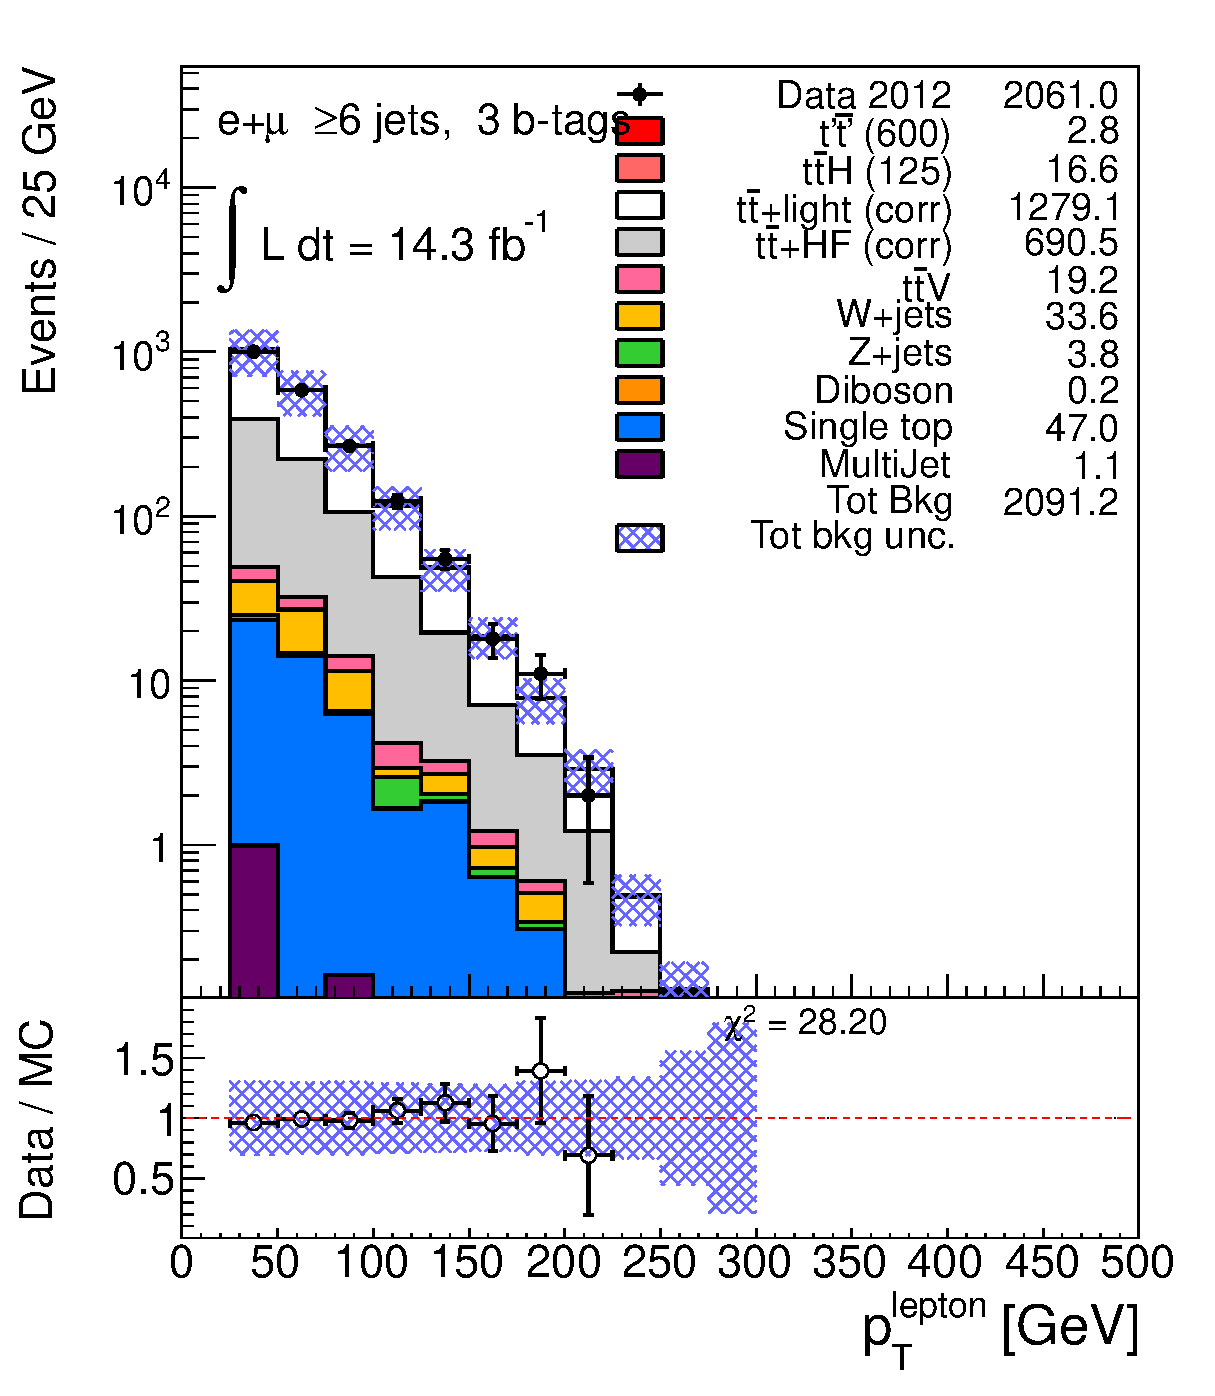
\includegraphics[width=0.30\textwidth]{figures/controlRegionsHTTail/LepPt_ELEMUON_6jetin3btagex_NOMINAL_logscale.eps} \\
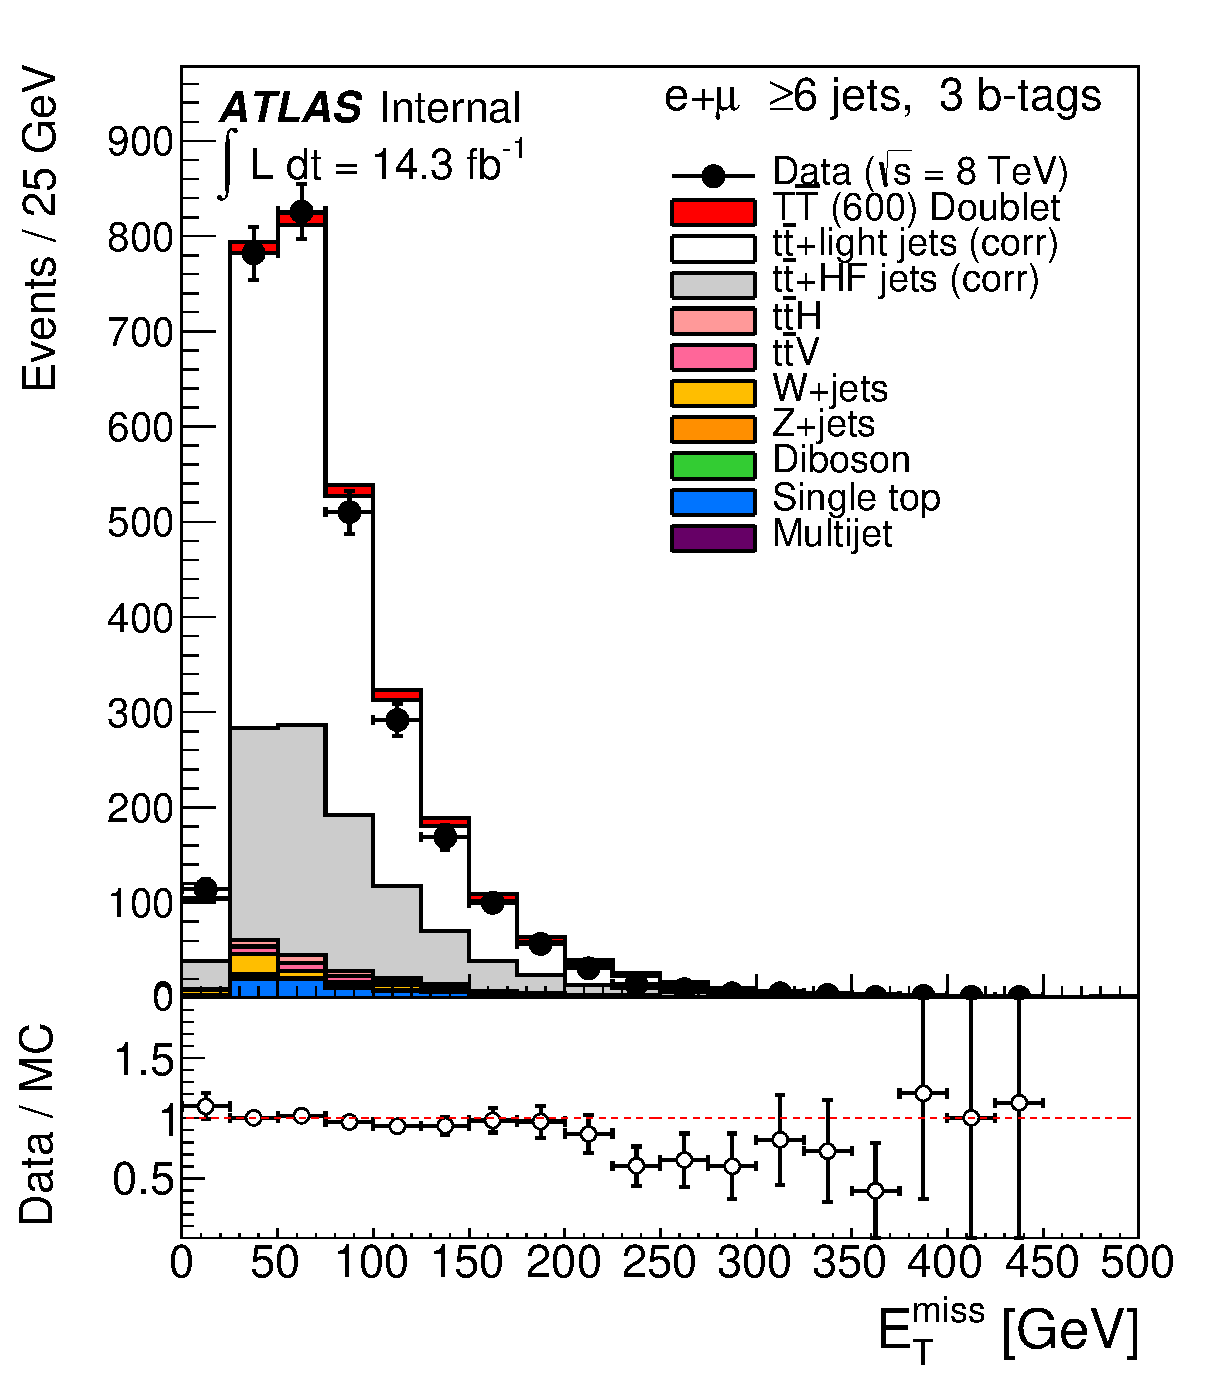
\includegraphics[width=0.30\textwidth]{figures/controlRegionsHTTail/MET_ELEMUON_6jetin3btagex_NOMINAL.eps} &
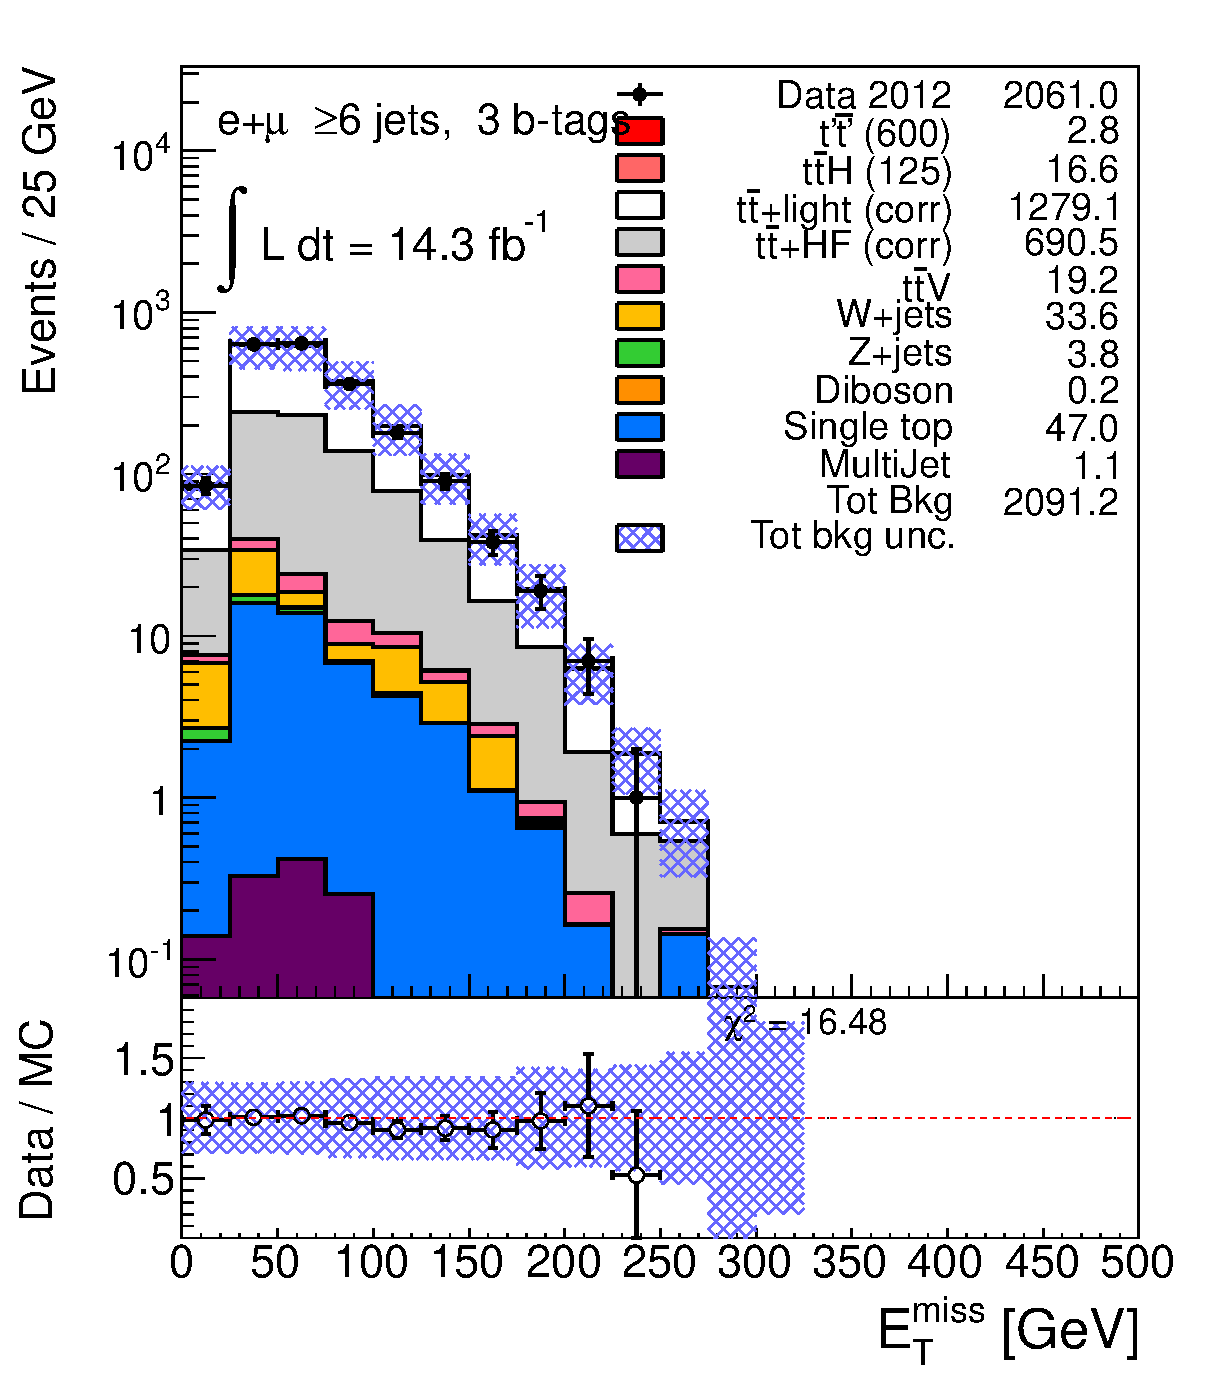
\includegraphics[width=0.30\textwidth]{figures/controlRegionsHTTail/MET_ELEMUON_6jetin3btagex_NOMINAL_logscale.eps} \\
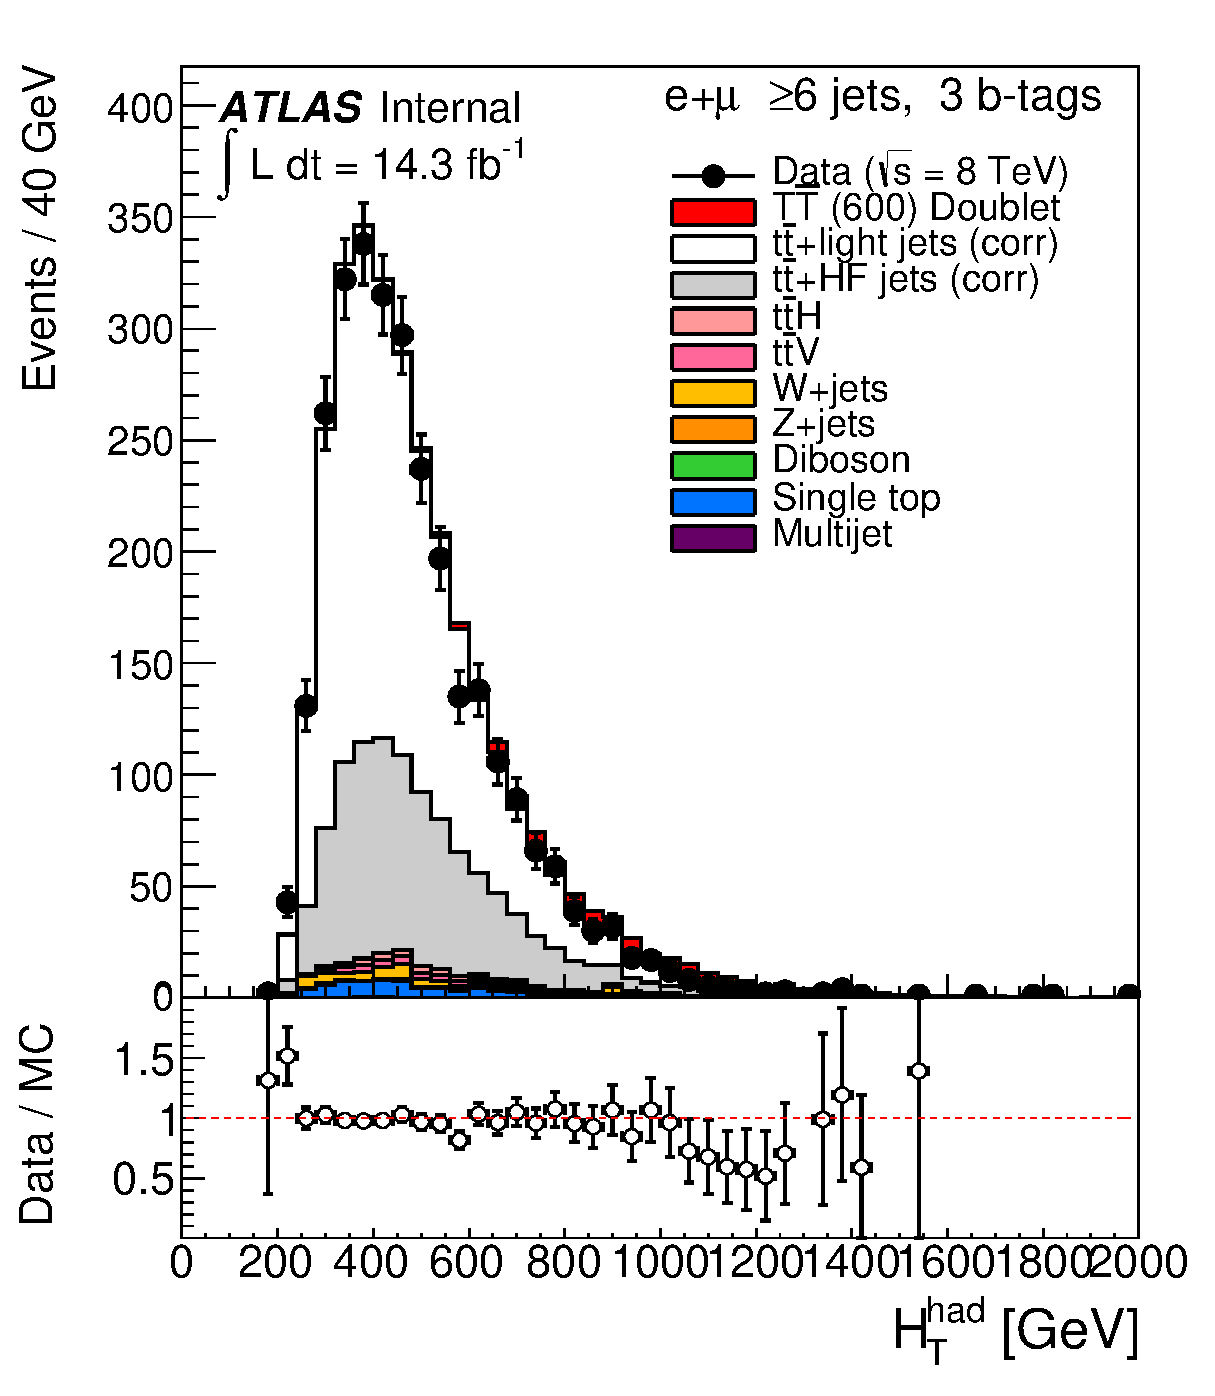
\includegraphics[width=0.30\textwidth]{figures/controlRegionsHTTail/HTHad_ELEMUON_6jetin3btagex_NOMINAL.eps} &
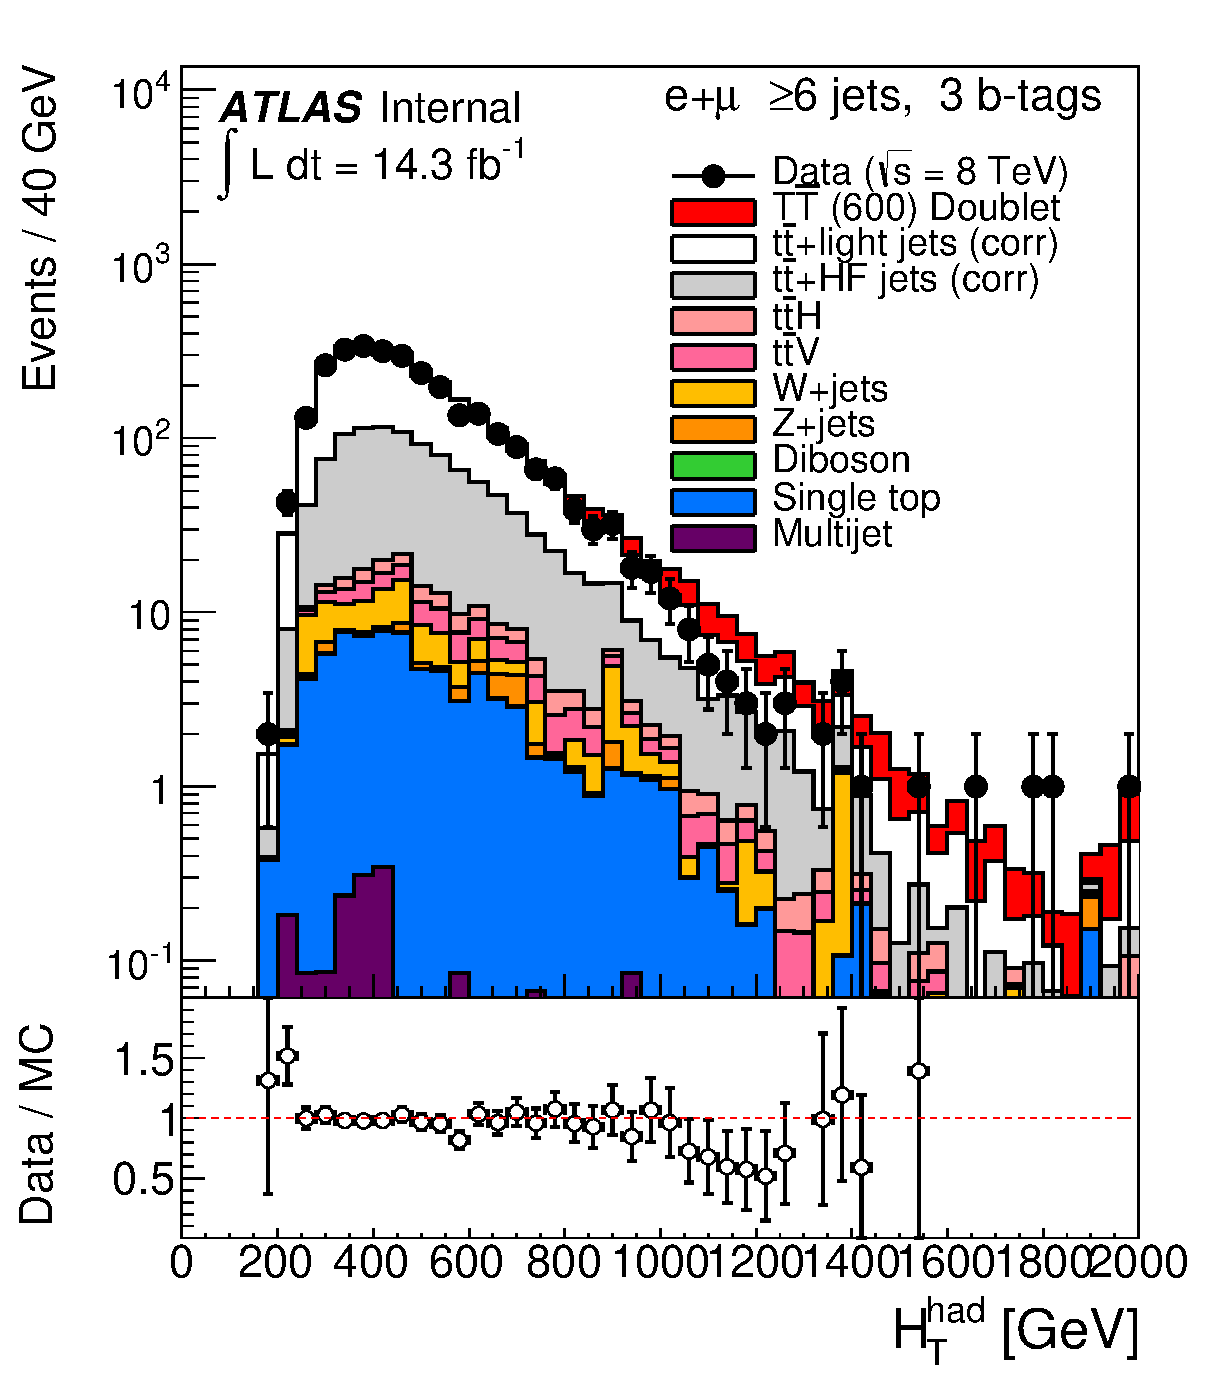
\includegraphics[width=0.30\textwidth]{figures/controlRegionsHTTail/HTHad_ELEMUON_6jetin3btagex_NOMINAL_logscale.eps} \\

\end{tabular}\caption{\small {Comparison between data and prediction in the combined $e$+jets and $\mu$+jets channels with 3 $b$-tagged jets in the control sample
defined to study the high $\HT$ tail (see text for details)  for a number of kinematic
variables. From top to bottom, the variables displayed are: $\HT$, and its basic ingredients, lepton $\pt$, $\met$ and $\hthad$,
in (left) linear scale and (right) logarithmic scale.
The shaded area represents the pre-fit total background uncertainty.}}
\label{fig:ELEMUON_controlHTTail_3btagex_1}
\end{center}
\end{figure}
%%%%%%%%%%%%%%
%%%%%%%%%%%%%%
\begin{figure}[htbp]
\begin{center}
\begin{tabular}{cc}
%
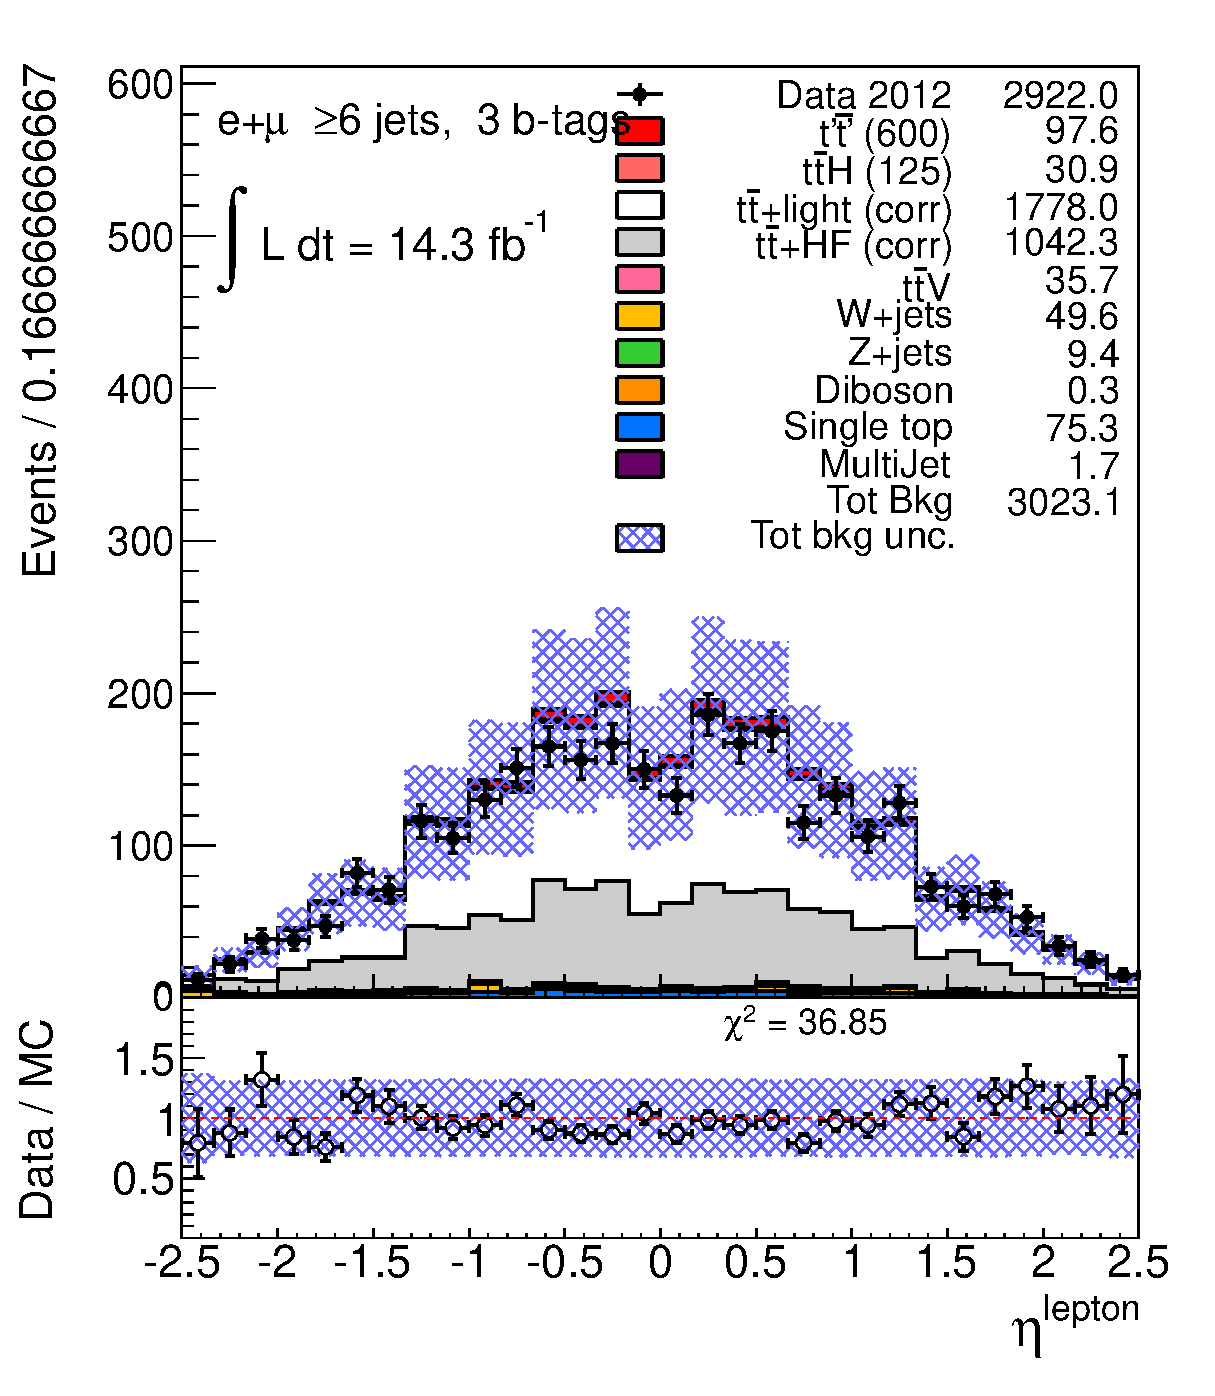
\includegraphics[width=0.30\textwidth]{figures/controlRegionsHTTail/LepEta_ELEMUON_6jetin3btagex_NOMINAL.eps} &
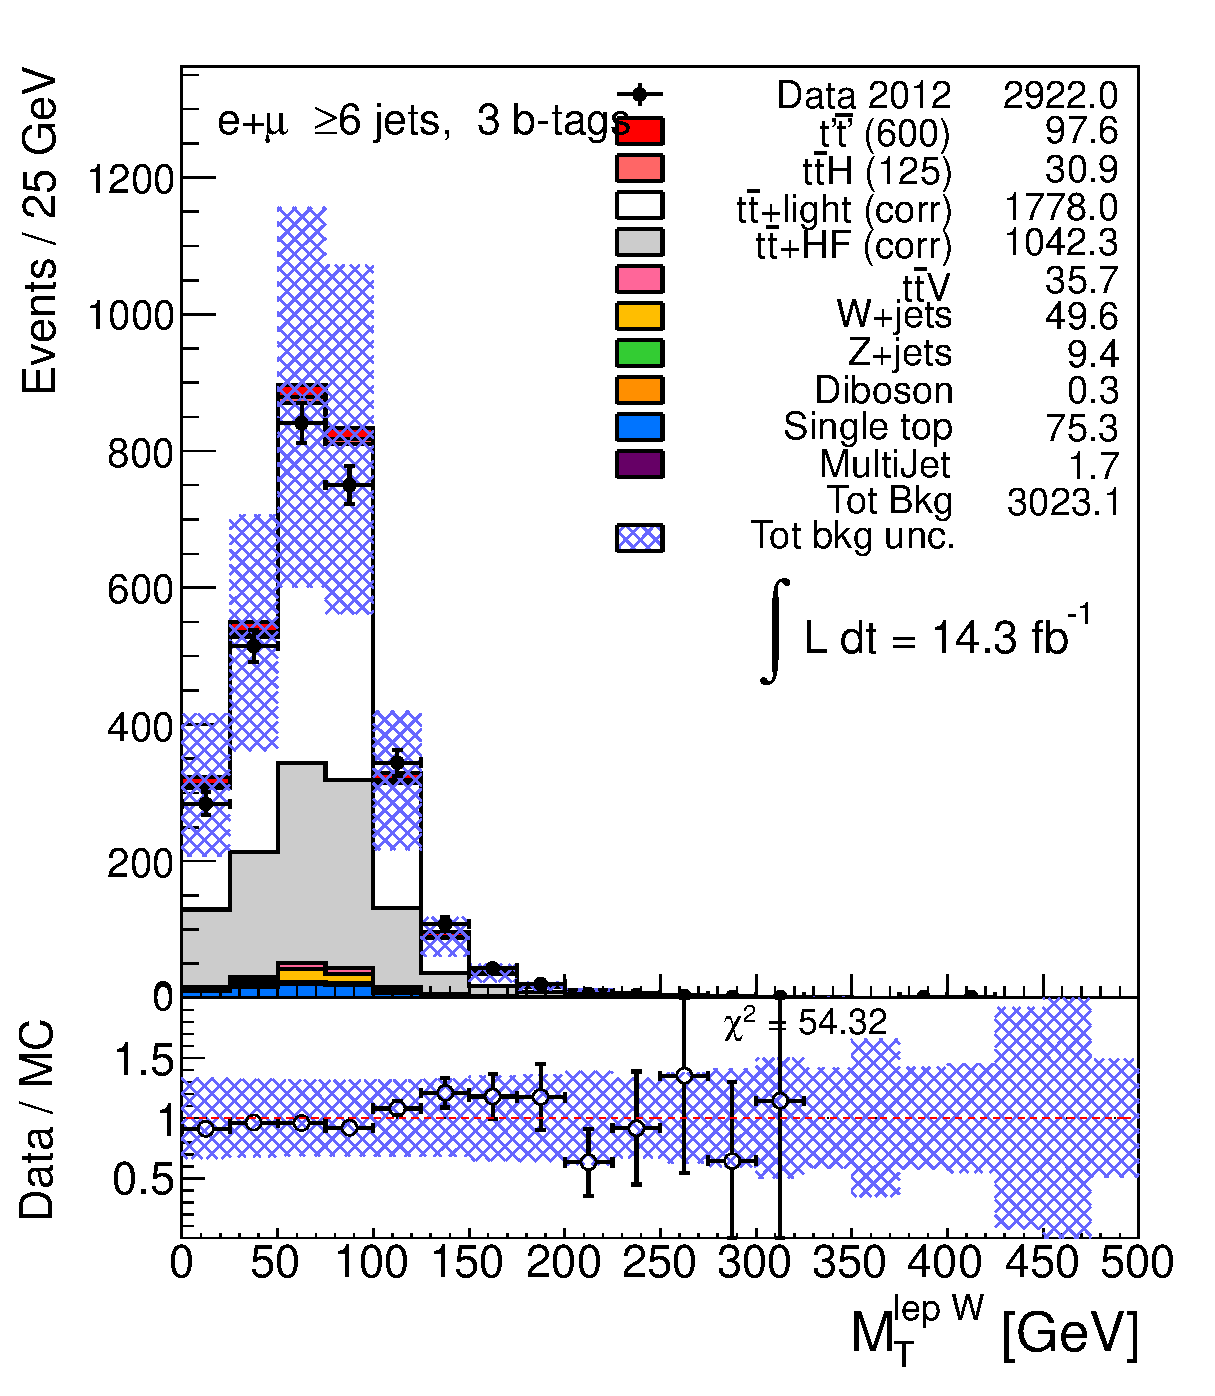
\includegraphics[width=0.30\textwidth]{figures/controlRegionsHTTail/Wlep_MassT_ELEMUON_6jetin3btagex_NOMINAL.eps} \\
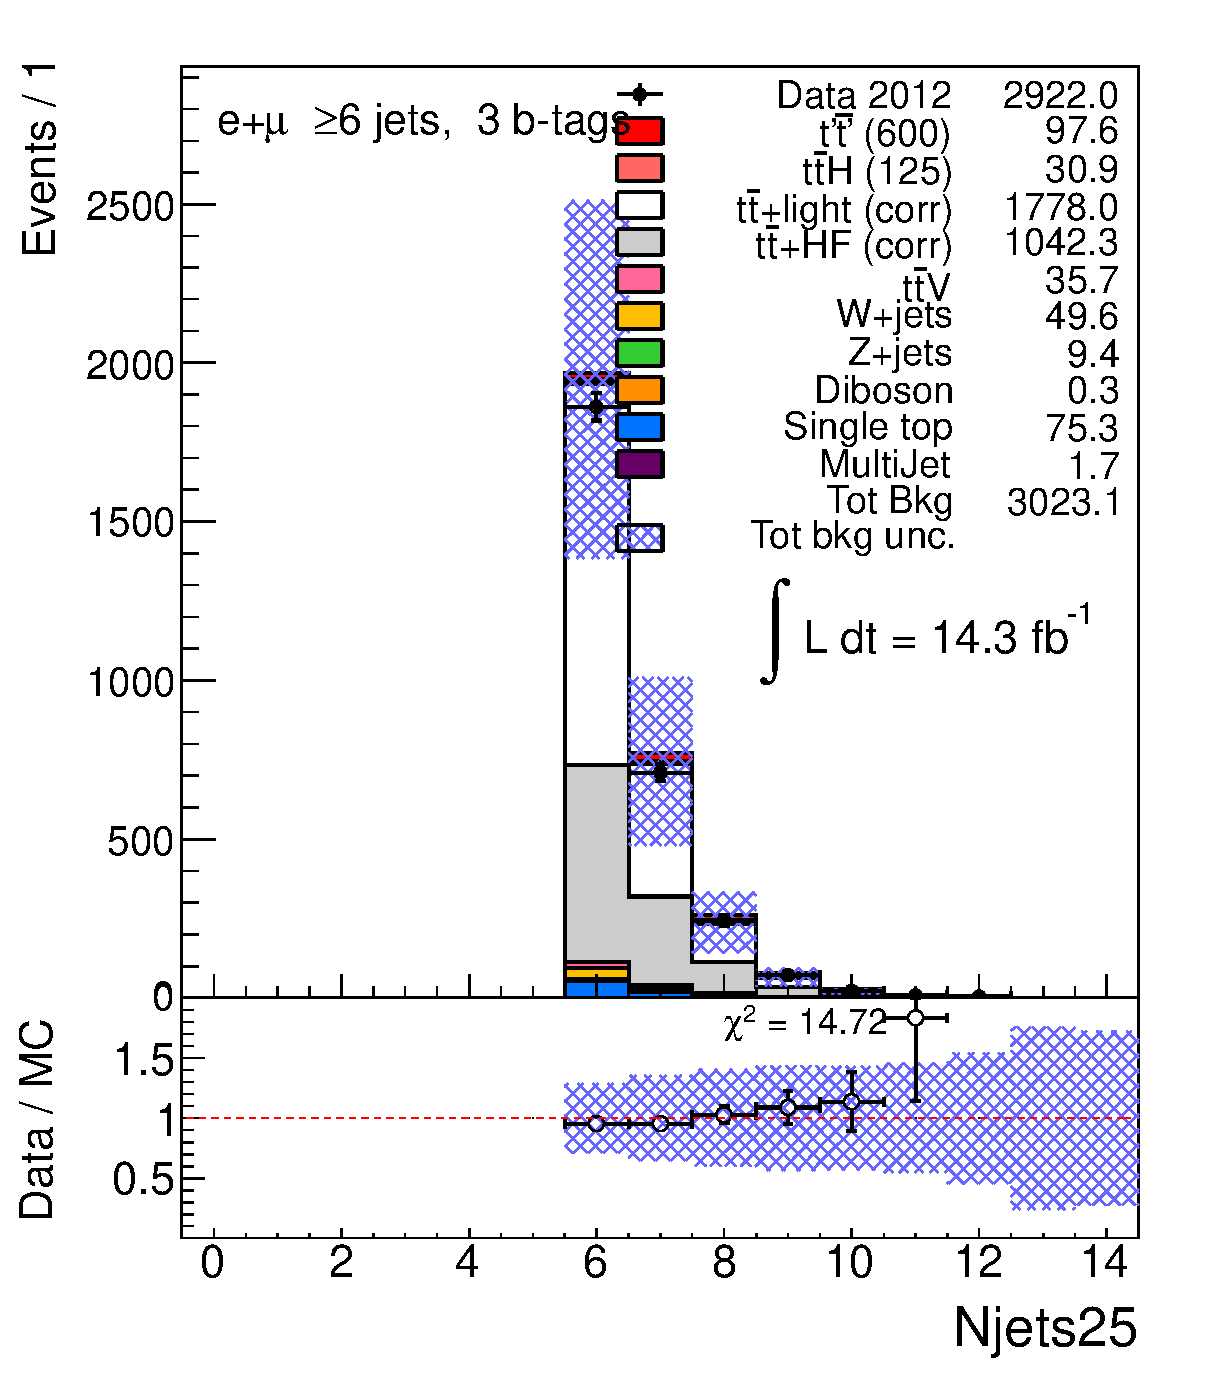
\includegraphics[width=0.30\textwidth]{figures/controlRegionsHTTail/Njets25_ELEMUON_6jetin3btagex_NOMINAL.eps} &
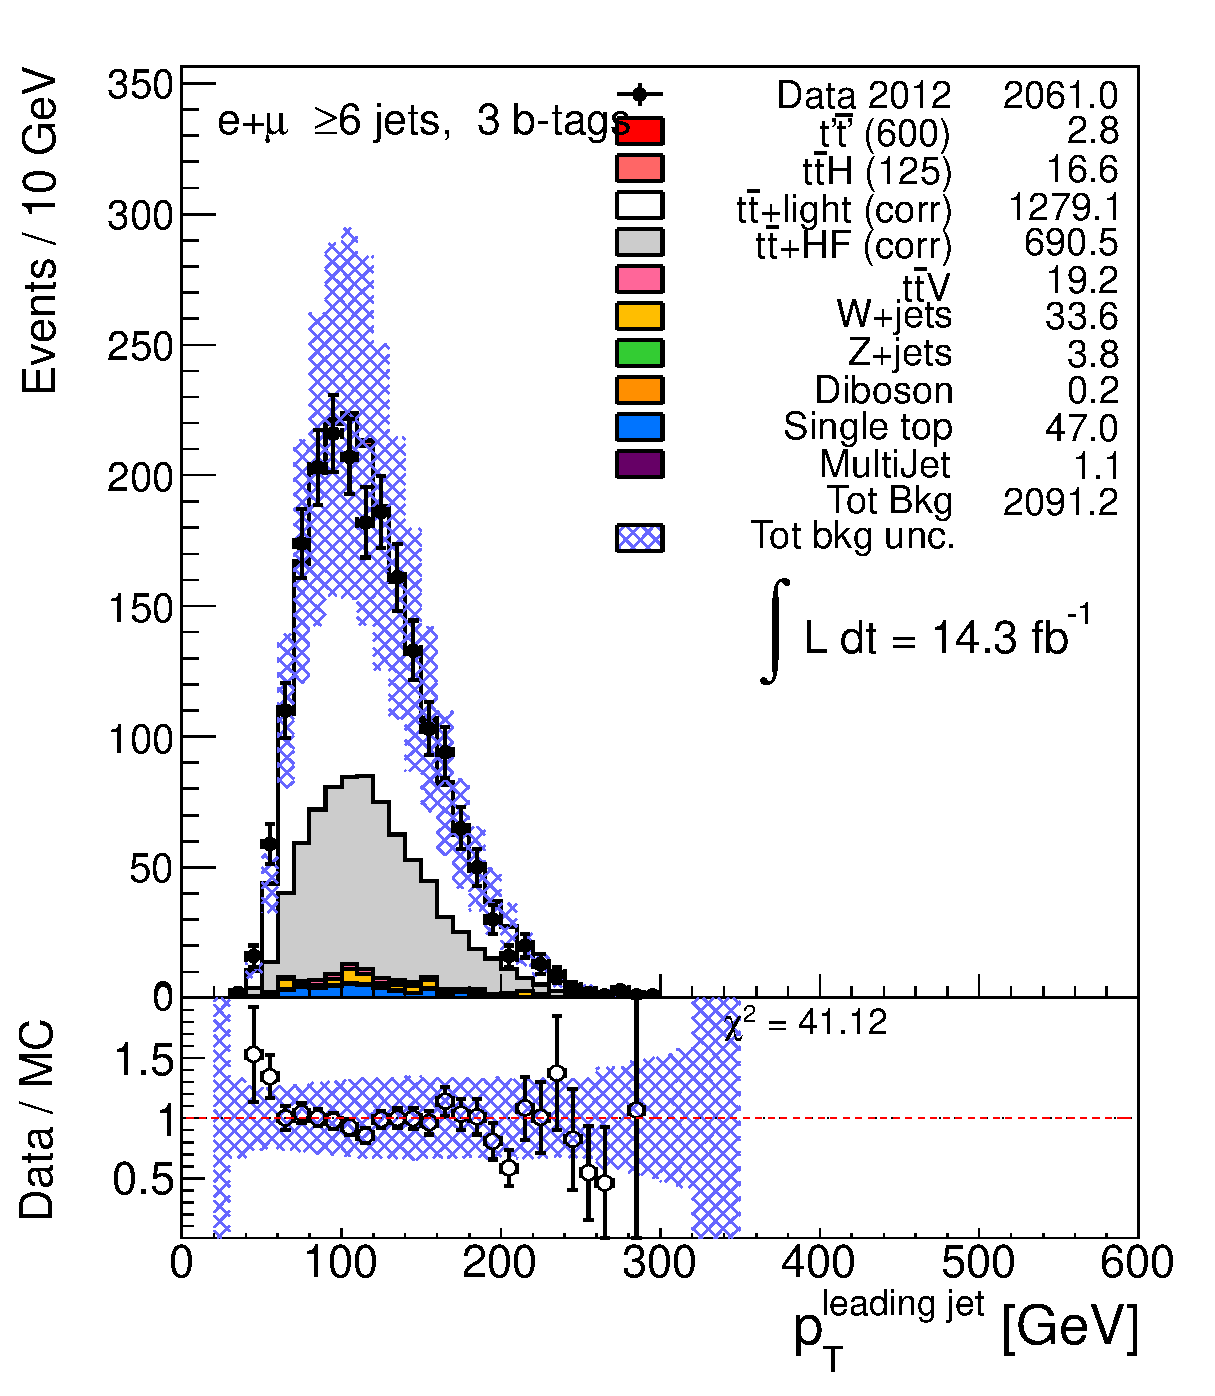
\includegraphics[width=0.30\textwidth]{figures/controlRegionsHTTail/JetPt1_ELEMUON_6jetin3btagex_NOMINAL.eps} \\
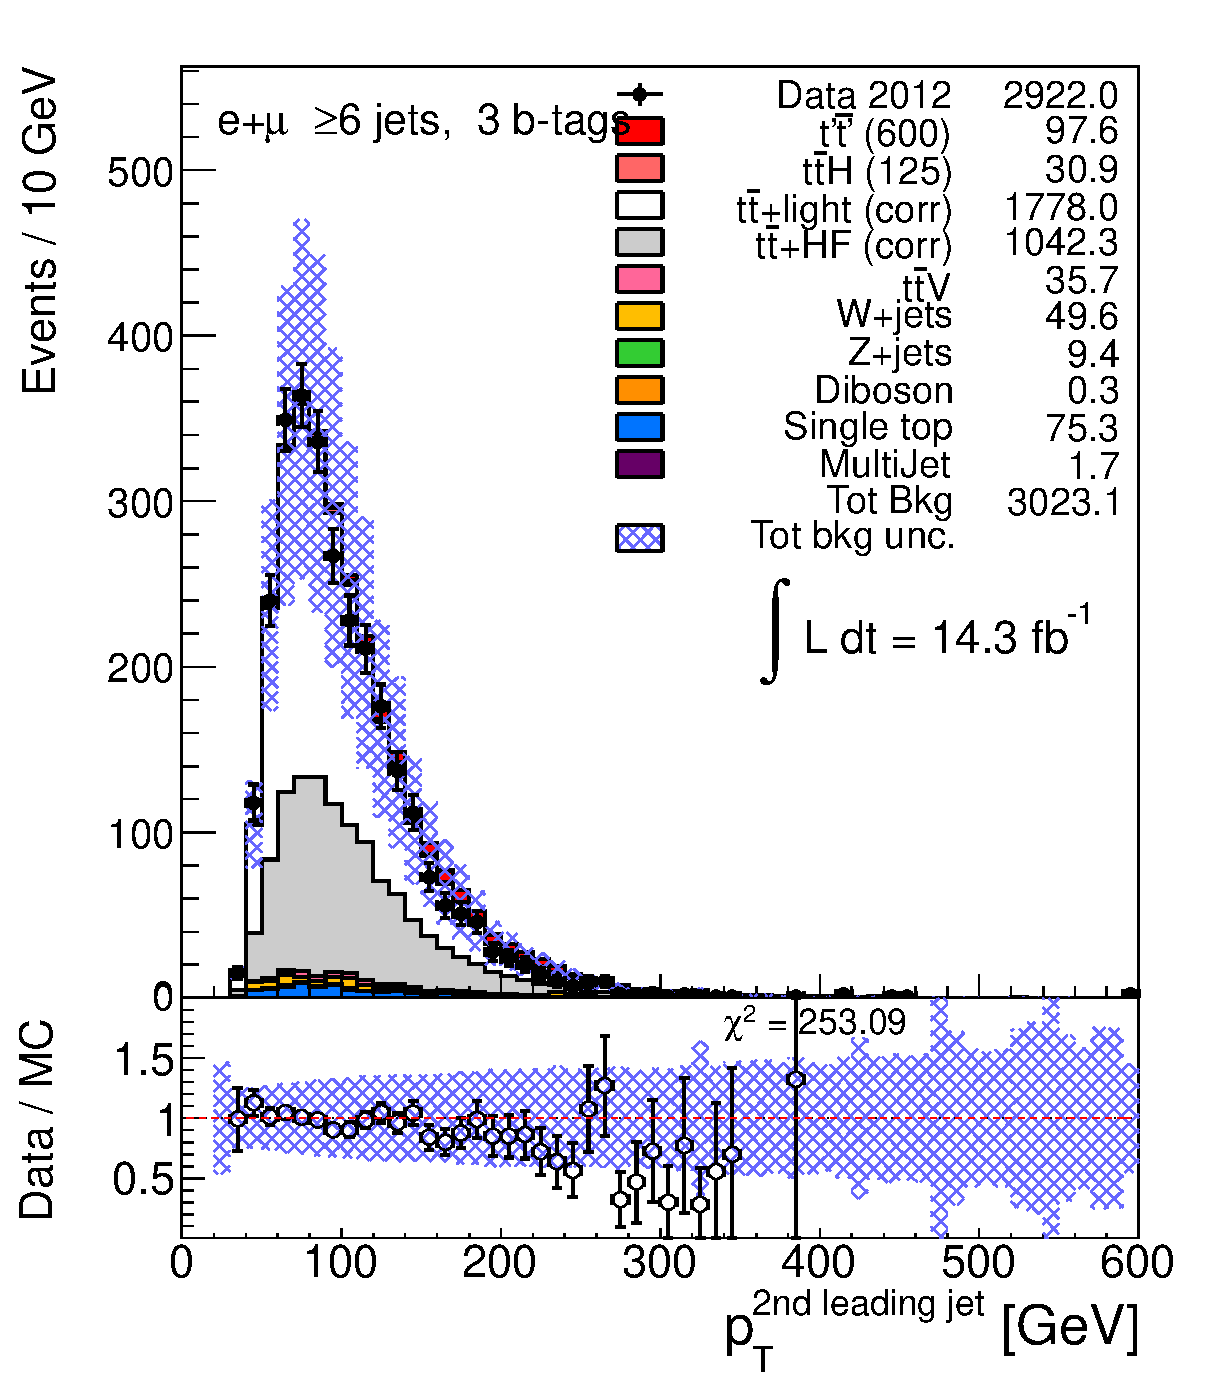
\includegraphics[width=0.30\textwidth]{figures/controlRegionsHTTail/JetPt2_ELEMUON_6jetin3btagex_NOMINAL.eps} &
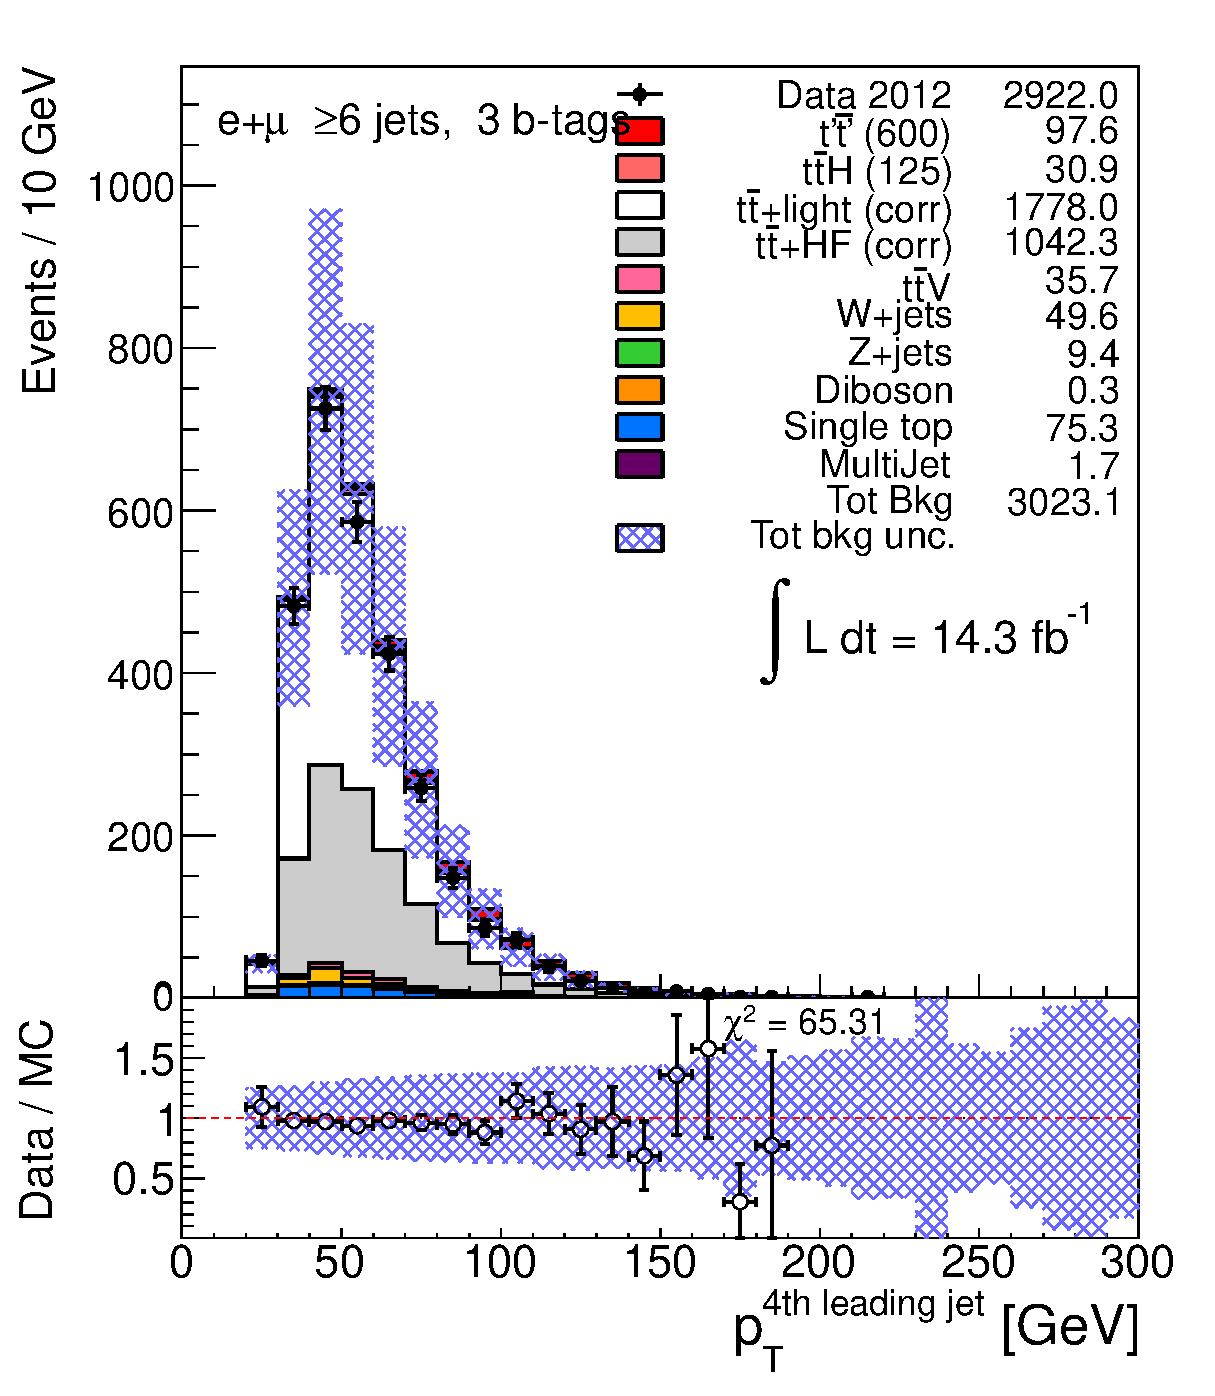
\includegraphics[width=0.30\textwidth]{figures/controlRegionsHTTail/JetPt4_ELEMUON_6jetin3btagex_NOMINAL.eps} \\
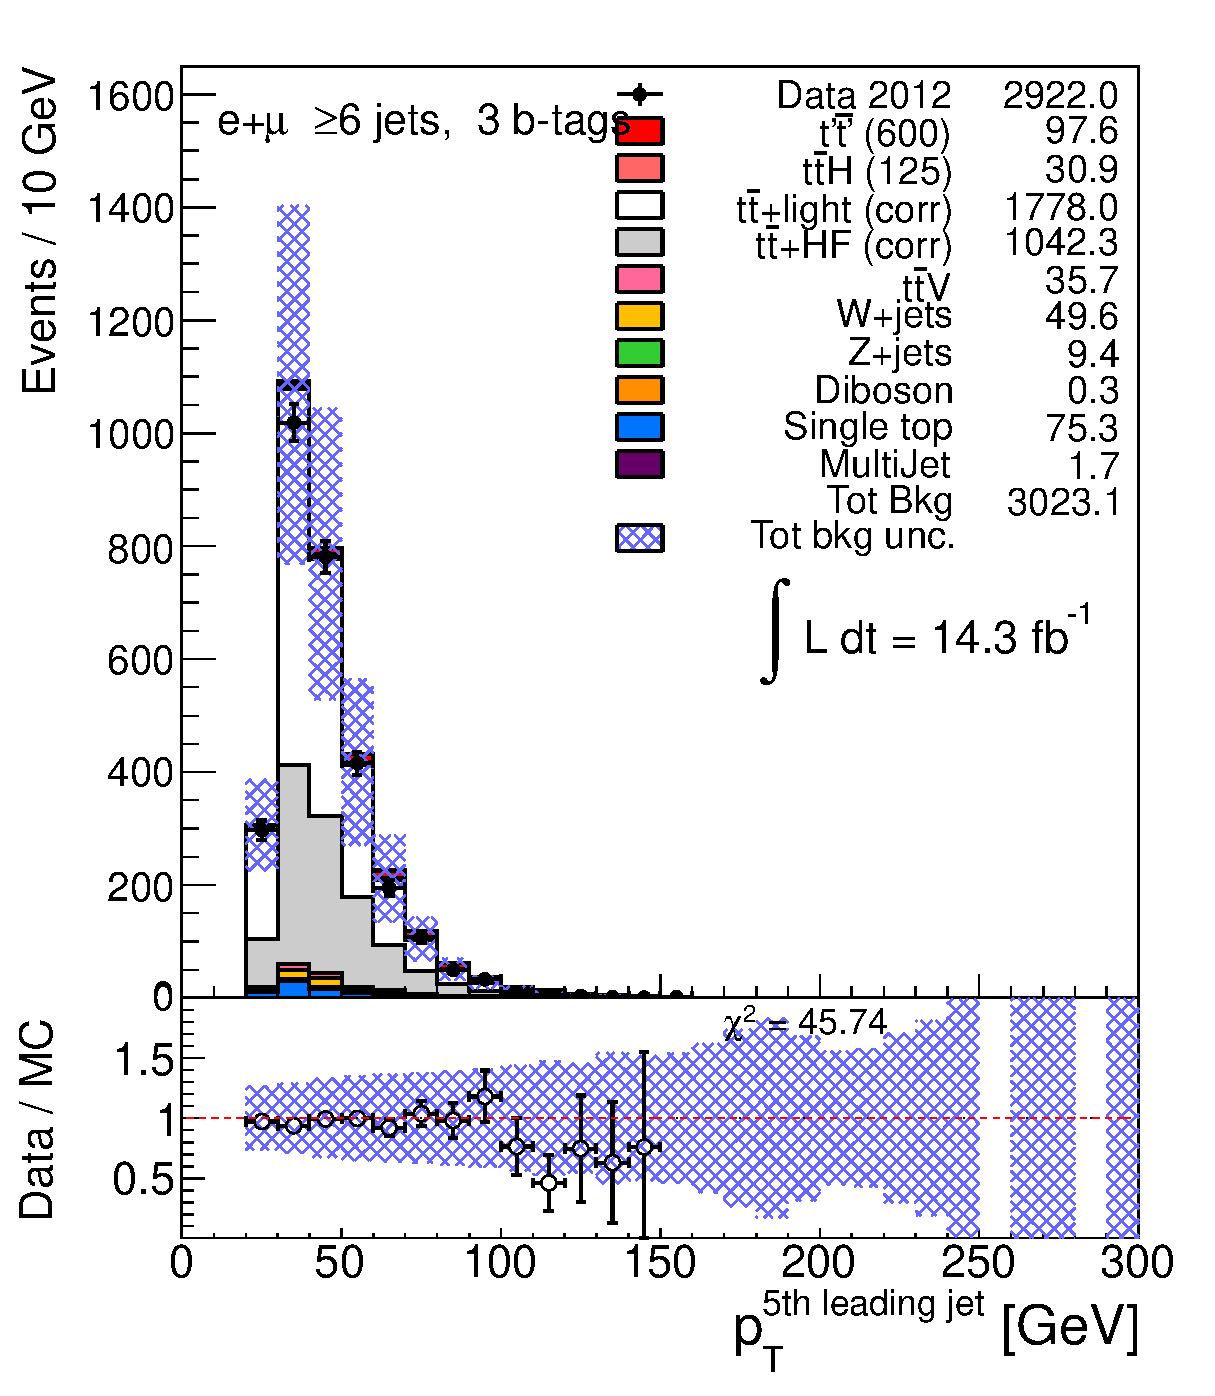
\includegraphics[width=0.30\textwidth]{figures/controlRegionsHTTail/JetPt5_ELEMUON_6jetin3btagex_NOMINAL.eps} &
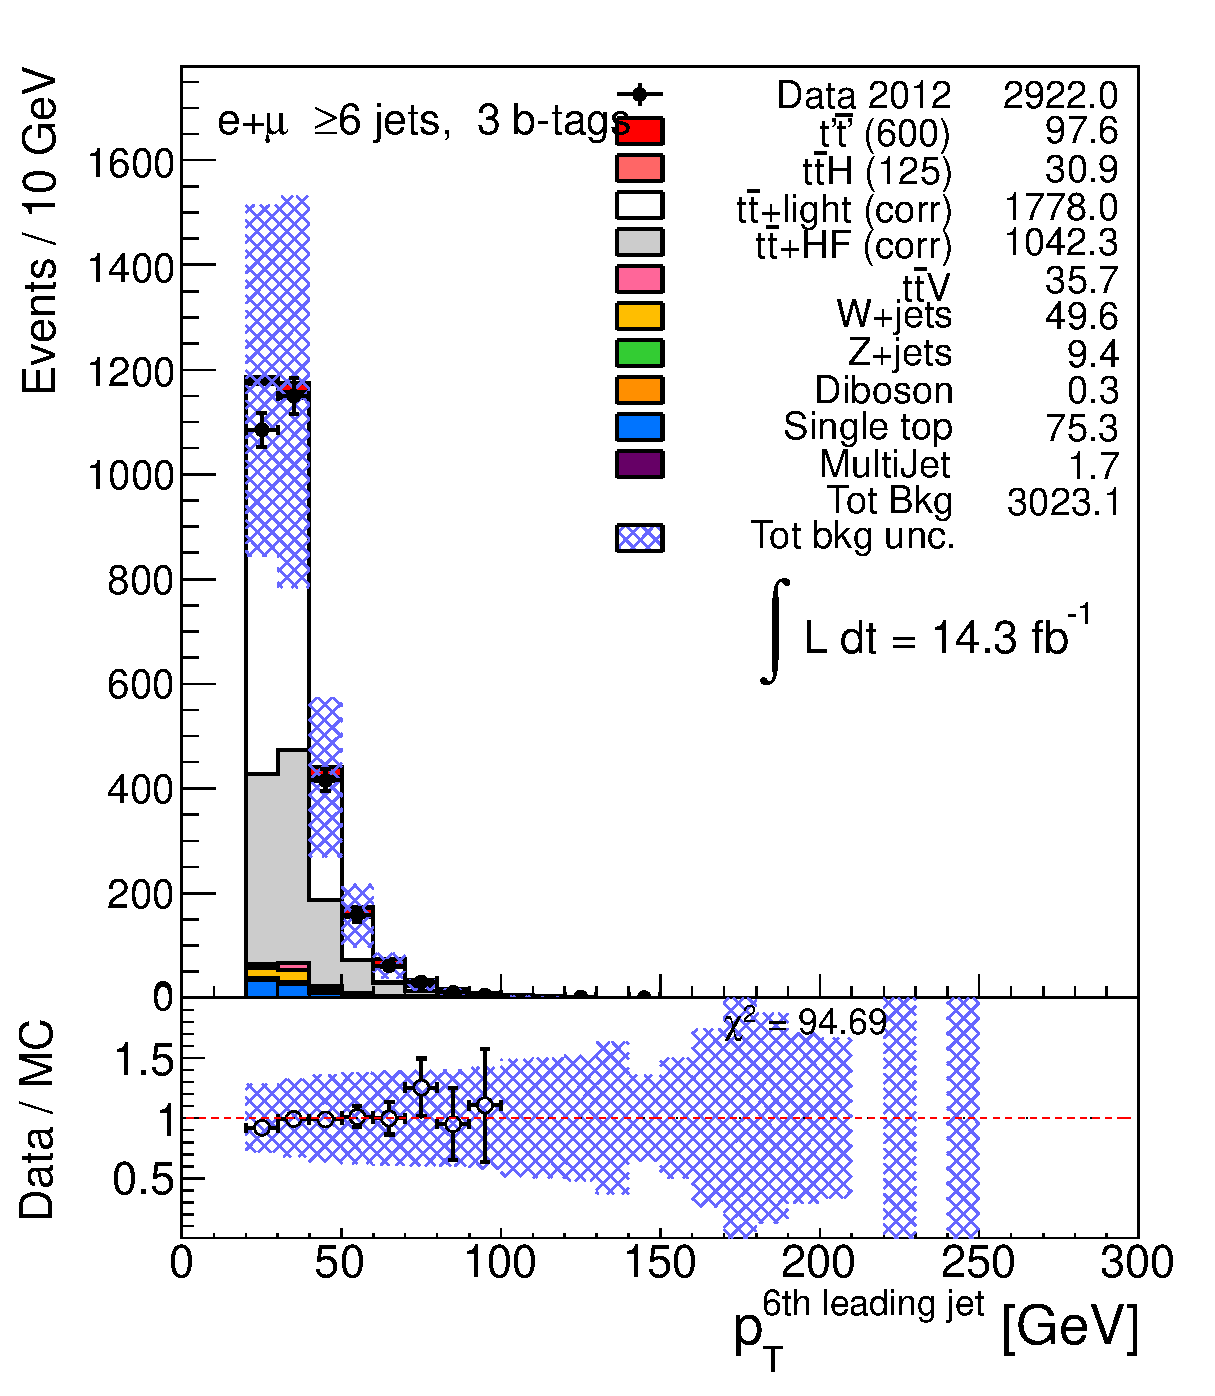
\includegraphics[width=0.30\textwidth]{figures/controlRegionsHTTail/JetPt6_ELEMUON_6jetin3btagex_NOMINAL.eps} \\
\end{tabular}\caption{\small {Comparison between data and prediction in the combined $e$+jets and $\mu$+jets channels with 3 $b$-tagged jets in the control sample
defined to study the high $\HT$ tail (see text for details)  for a number of kinematic
variables. From top to bottom, and left to right, the variables displayed are: lepton $\eta$, $W$ transverse mass, jet multiplicity with $\pt>25\gev$, 
and jet $\pt$ up to the 6th leading jet.
The shaded area represents the pre-fit total background uncertainty.}}
\label{fig:ELEMUON_controlHTTail_3btagex_2}
\end{center}
\end{figure}
%%%%%%%%%%%%%%
